%!TeXroot=../main.tex

\chapter{区块链上隐私保护技术分析}
\label{chap:privacy}

在区块链系统的实际使用中,为了保证区块链上记录数据的可溯源、可验证等特性,所有数据都必须公开给区块链网络中的所有节点。这一特性在保障安全、可验证的同时,导致恶意攻击者可以直接获取区块链账本中记录的数据,并通过分析数据窥探用户隐私。攻击者通过分析区块链账本中记录的交易数据,发掘其中规律,将用户的不同地址、交易数据关联,并进一步对应到用户的现实身份[7-14]。这类分析攻击主要分为地址聚类和身份定位两阶段。地址聚类阶段根据用户行为特征将可能属于同一用户的地址、交易进行聚类,得到地址间关联关系。身份定位阶段搜集与区块链地址相关联的用户信息,例如论坛、交易所等服务记录的与链上地址对应的手机、邮箱、IP地址等用户链下信息,再根据搜集到的信息确定用户身份,关联该用户所有地址与交易信息,揭露该用户的所有历史记录。

近年来,许多研究者开始关注区块链系统中的隐私问题,该领域中相应的防御技术也不断出现。在区块链隐私分析上,祝烈煌等人从身份隐私和交易隐私两方面分析区块链中的隐私问题,身份隐私指用户身份信息和区块链地址之间的关联关系,交易隐私指区块链中存储的交易记录及背后的知识。Sarah等人提出用抗追溯性来度量区块链中用户信息的匿名性。本文从账本存储和网络通信两个方面,分析区块链系统中隐私信息可能泄露的内容和方式。从账本存储角度,需要保护用户存储在区块链账本上的数据记录所包含的隐私信息;从网络通信角度,需要保护区块链网络中的节点隐私及网络通信中的流量等隐私信息。在隐私保护技术方面,祝烈煌等人[30]从网络层、交易层和应用层出发分别描述区块链隐私保护面临的威胁以及采用的保护技术。Merve等人和李旭东等人将研究分为两大类:基于比特币系统的研究和针对比特币系统进行拓展和替换的研究。

本章对比特币系统以外的区块链隐私保护技术进行更大范围的技术介绍与对比。主要通过技术实现原理,将保护技术划分为地址混淆,信息隐藏和通道隔离,并对各类技术抽象出通用模型,然后介绍各类隐私保护技术的实现及对比。其中地址混淆机制通过交易交换不同用户的资产,对同一用户不同地址间的关联关系进行混淆,从而破坏地址聚类的假设前提;信息隐藏机制通过零知识证明、同态加密等密码学技术加密区块链账本中记录的隐私信息,同时保持账本正确性的可验证;通道隔离机制在区块链网络中设置访问权限,将需要权限访问的数据保护在特定通道中。

\section{区块链隐私及威胁}

传统的区块链系统中通常采用假名机制和广播机制保护用户隐私。其中假名机制指用户可以独立生成任意数量的区块链地址,不需要通过注册或者认证机制。同一用户生成的不同地址可以单独使用,彼此间不存在任何关联关系。因此,仅通过区块链地址无法关联到用户的真实身份,该机制能隔离用户在区块链上不同操作的记录。广播机制指区块链系统通过p2p网络传输数据,网络中采用洪水广播协议传播消息,接受节点无法判断消息来源是消息的直接发起者还是转发者,从而保护消息真实发起者的身份。

假名机制和广播机制能在一定程度上保护区块链用户的隐私安全。但在实际应用中,用户隐私仍面临各类威胁,主要存在于记录数据的分布式账本和区块链去中心化网络中各节点的相关信息。为了保证去中心化系统的正确性和安全性,区块链系统中的所有节点共同维护一致的分布式账本,记录区块链系统中的所有历史数据,用于验证用户提交的新事务的合法性。为了所有节点都能验证账本的正确性,账本中所有数据保持公开,因此账本数据能被攻击者轻易获取,攻击者通过分析公开账本中的记录严重威胁用户隐私。此外,区块链系统采用去中心化网路进行通信,在非许可链系统中,节点加入网络不需要任何身份认证,这在增强了扩展性的同时也导致攻击者可以自由部署节点加入网络,监听网络中各节点隐私信息以及网络中通信信息。本章围绕这两部分介绍需要保护的隐私内容及对应的威胁方式。

\subsection{账本隐私及威胁}

区块链账本记录了区块链系统中的各类事务数据,由于目前区块链系统主要应用于密码货币领域,因此区块链账本主要记录交易数据。交易模型主要分为未花费交易输出(UTXO,UnspentTransactionOutput)模型和账户(Account)模型两类[34]。部分攻击方式针对特定的交易模型,例如交易网络构造攻击和资产追踪攻击针对UTXO模型。账本隐私主要包含以下内容:
交易内容隐私:账本记录的单笔交易内容,包含交易发起方、交易接受方、交易金额以及附带数据等隐私信息。
账户地址隐私:区块链地址与交易的关联关系,包含账户地址的交易记录、账户余额以及不同账户地址间交易关联等隐私信息。
用户身份隐私:用户和区块链地址、交易的关联关系,包含同一用户的交易记录、资金余额等隐私信息。
在区块链系统的实际应用中,用户常需要发起多输入交易,即存在多个输入资产的交易。该交易需要每个输入地址的签名,可以由一个或多个用户生成。由于多个用户对同一交易进行签名的过程较为复杂,通常多输入交易由同一用户生成。此外,在基于UTXO模型的交易系统中,未花费资产只能使用一次,因此当花费资产超过交易所需资产时,用户将超出部分的资产转移到自己的另一账户地址中。用于接受超出部分资产的账户地址通常称为找零地址。针对账本隐私包含的各类隐私,目前的主要攻击方式为账本分析攻击,通过分析区块链账本数据,利用用户常见的交易规律,构建账户地址与交易之间以及用户与账户地址之间的一对多对应关系,威胁账本地址隐私与用户身份隐私。攻击者根据区块链系统的设计与上述使用特征提出以下假设:

\begin{enumerate}
	\item 假设1 多输入交易的所有输入地址为同一用户所持有。
	\item 假设2 交易的找零地址和输入地址为同一用户所持有。
\end{enumerate}

2013年,Reid等人下载了比特币系统2009年1月3日至2011年7月12日的全部账本数据,通过分析数据首先构建交易网络。交易网络中节点表示单次交易,节点间的有向边为交易间的输出-输入对,表示前一次交易的输出作为后一次交易的输入,每条边同时记录了交易金额以及交易时间。部分交易网络如图\ref{fig:sub-network}所示。

\begin{figure}
\centering
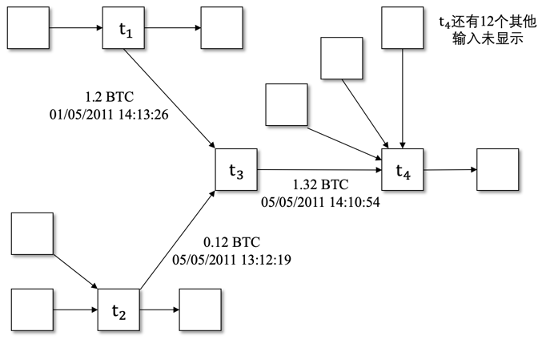
\includegraphics[height=7cm]{figures/sub-network.png}
\caption{交易网络示例}
\label{fig:sub-network}
\end{figure}

在交易网络的基础上,提取所有多输入交易,构建账户地址间的非完全网络。如图\ref{fig:nc-user-network}所示,非完全网络中节点表示地址,节点间有向边表示地址间交易的时间和金额。Reid等人根据中本聪提到的多输入交易关联风险提出假设1,即假设多输入交易的所有输入地址为同一用户所有。基于这一假设,在非完全网络的基础上,可以聚合属于同一用户的所有地址,进而构建用户网络,用户网络中节点表示一个用户,节点间的有向边表示用户间资产流动信息。

\begin{figure}[ht]
  \centering%
  \subcaptionbox{非完全网络中的局部示例\label{fig:nc-network}}
    {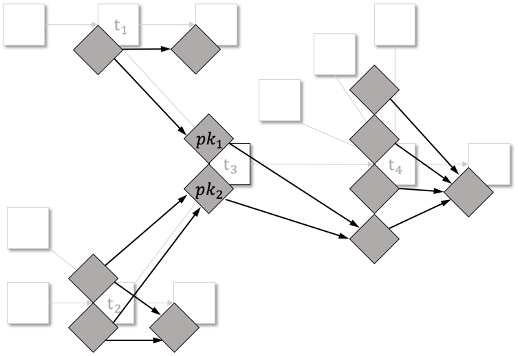
\includegraphics[height=7cm]{figures/nc-network.png}}%
  \hspace{4em}%
  \subcaptionbox{用户网络中的局部示例\label{fig:user-network}}
      {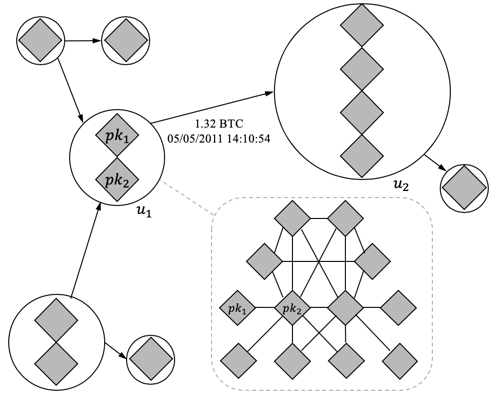
\includegraphics[height=7cm]{figures/user-network.png}}
  \caption{非完全网络与用户网络示例}
  \label{fig:nc-user-network}
\end{figure}

2013年,Androulaki等人[8]根据区块链钱包的应用特征提出了挖掘找零地址的方法,如果一个交易拥有两个输出,其中一个为已出现过的地址,另一个为新地址,则将新地址视为找零地址,并提出了假设2,即交易的找零地址和输入地址为同一用户所持有。为了验证假设的正确性,Androulaki等人在大学中构建了模拟的密码货币使用环境,通过搜集用户使用记录,并利用假设1和假设2进行分析,挖掘出40\%左右用户的真实身份。受此启发,Meiklejohn等人[9]给出了“找零地址”更完善的定义:
	
找零地址如果交易t中的一个输出公钥地址pk满足以下所有特征,则可将pk视为“找零地址”。

\begin{enumerate}
	\item $d_{addr}^{+}(pk) = 1$该地址pk在非完全网络中入度为1,即在区块链账本中首次出现。
	\item 交易t为铸币交易以外的普通交易。铸币交易即生成新区块时发布奖励的交易。
	\item 不存在$pk^{'}\in  output(t)$且$pk^{'}\in  input(t)$,即不存在“自找零地址”。
	\item 不存在$pk^{'}\in  output(t)$,$pk^{'} \neq pk$且$d_{addr}^{+}(pk^{'}) = 1$,即pk为输出地址中唯一首次出现的地址。
\end{enumerate}

综上所述,账本隐私内容主要集中于单次交易的内容及隐藏在多个相关交易之后的用户身份、账户余额等隐私信息。这部分信息记录在公开的区块链账本中,攻击者可以通过分析账本挖掘出其中的关联信息,威胁用户的账本隐私。

\subsection{网络隐私及威胁}

区块链系统通过去中心化的P2P网络进行节点间通信,而在非许可链系统中的网络不存在准入限制,这在增强了扩展性的同时也带来了潜在的风险。攻击者可以任意部署节点,监听网络中各节点隐私信息以及网络通信信息,甚至尝试对正常节点发起攻击。区块链网络主要存在以下隐私内容:

\begin{description}
  \item[\textbf{节点隐私}] 节点自身的隐私内容,包含节点网络IP、软件版本、服务器系统等隐私信息。
  \item[\textbf{通信隐私}] 节点间通信隐私内容,包含节点间通信的数据内容以及通信流量情况。
\end{description}

2013年,Reid等人尝试利用BitcoinFaucet公开的区块链地址及IP地址对应关系进行分析,揭露比特币用户与实际物理位置的对应关系,该尝试只涉及到很少的节点。Bitnodes网站通过部署大量节点,探测全球范围内的比特币节点信息,其中IP地址分布信息如图\ref{fig:bitcoin-dis}所示(截图于2019年08月01日)。

\begin{figure}
\centering
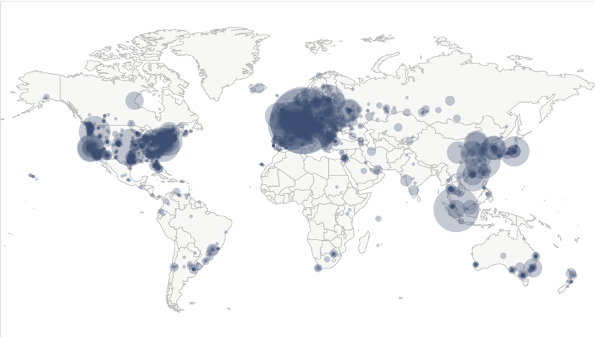
\includegraphics[height=7cm]{figures/bitcoin-dis.png}
\caption{世界范围内比特币节点分布情况}
\label{fig:bitcoin-dis}
\end{figure}

探测攻击严重威胁节点隐私,更进一步,攻击者通过大量探测可以将区块链中广播的数据与实际发起节点关联,尽管区块链网络采用洪水广播的方式保护实际发起人,但是在布置大量探测节点后,攻击者有很大概率找出消息的真实发起节点。2011年,Kaminsky在黑帽大会上提出假设,假设第一次接受到消息时的来源节点即为该消息的真实发起节点。

\begin{figure}[ht]
  \centering%
  \subcaptionbox{模式1 单一转发者\label{fig:trans-pattern1}}
    {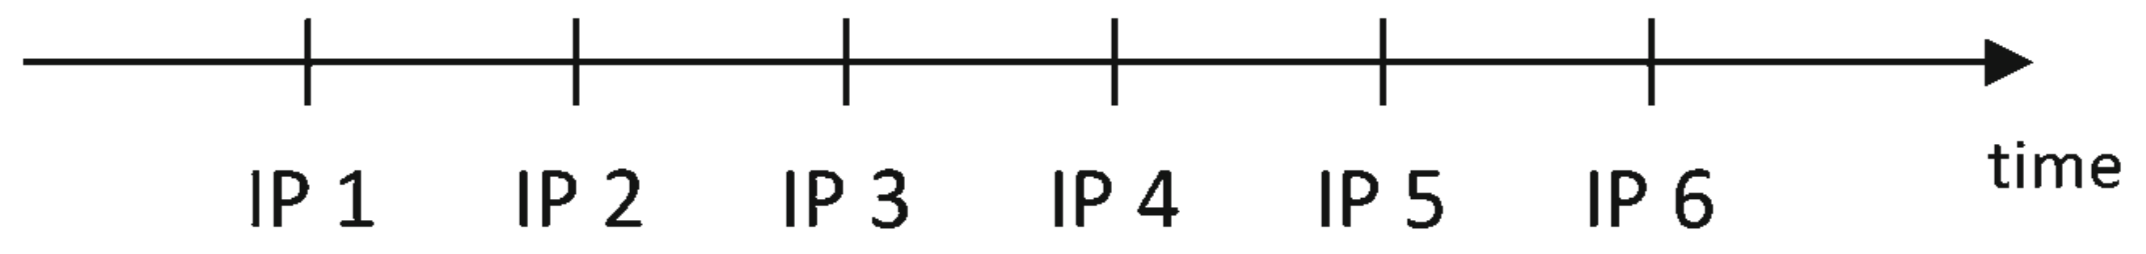
\includegraphics[width=7cm]{figures/trans-pattern1.png}}%
  \hspace{2em}%
  \subcaptionbox{模式2 多转发者,无重复转发者\label{fig:trans-pattern2}}
  	{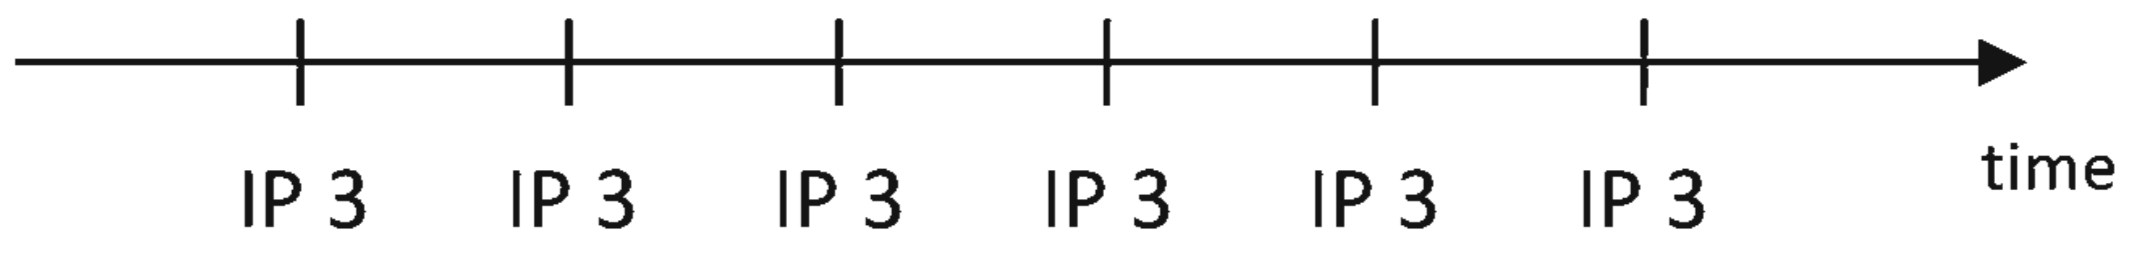
\includegraphics[width=7cm]{figures/trans-pattern2.png}}

  \subcaptionbox{模式3A 多转发者,单一重复转发者\label{fig:trans-pattern3}}
    {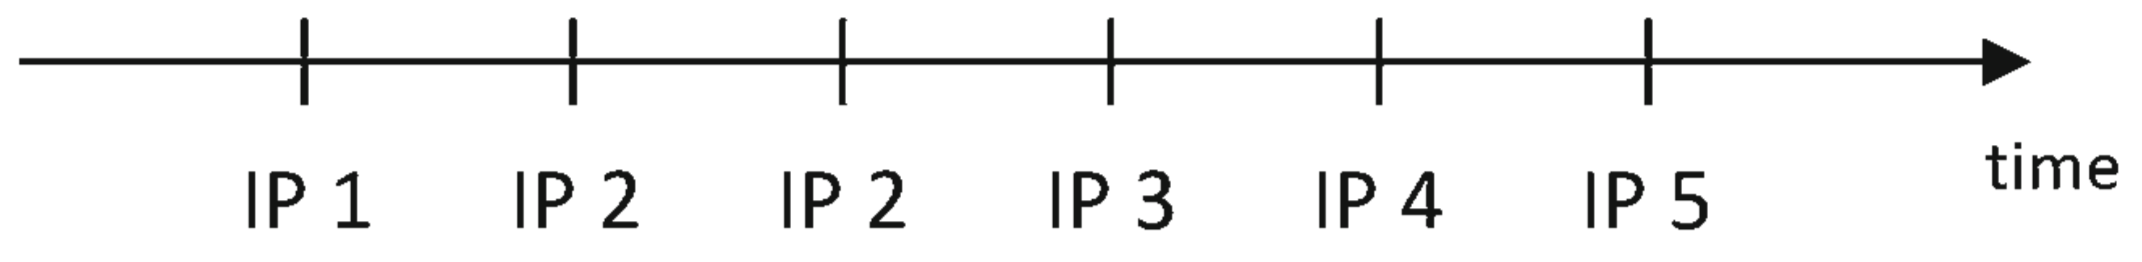
\includegraphics[width=7cm]{figures/trans-pattern3.png}}%
  \hspace{2em}%
  \subcaptionbox{模式3B 多转发者,多重复转发者\label{fig:trans-pattern4}}
  	{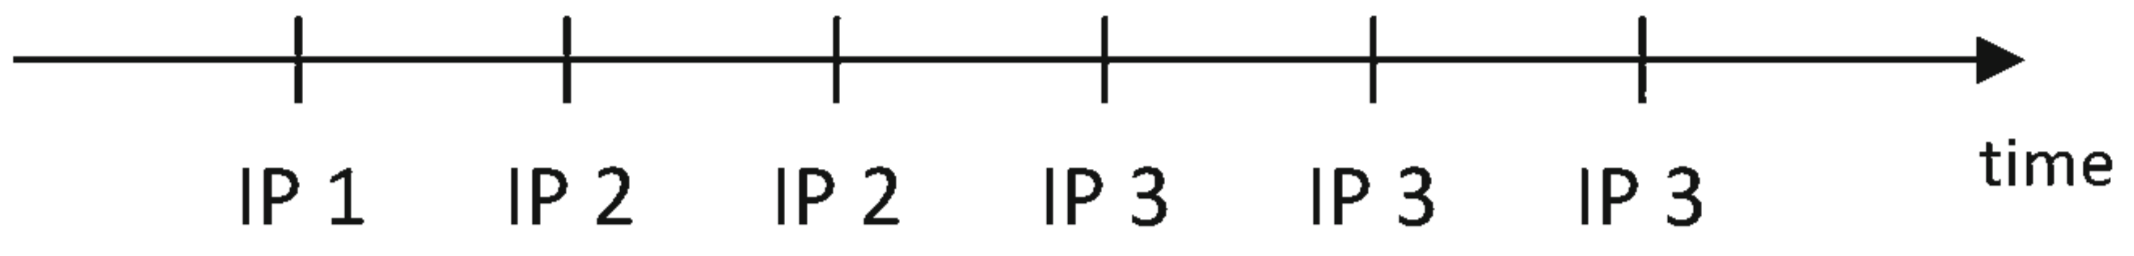
\includegraphics[width=7cm]{figures/trans-pattern4.png}}
  \caption{区块链网络中三种消息传播模式传播节点随时间的变化}
  \label{fig:trans3}
\end{figure}

2014年,Koshy等人在Kaminsky所提出假设的基础上进行了完善,归纳一段时间内监听到的消息传播情况,提出了区块链网络中消息传播的四种模式(如图\ref{fig:trans3}所示)以及对应的真实发起者假设。这一攻击方式通过监听消息传播模式,分析真实发起节点,将IP地址与消息中包含的链上地址对应,威胁通信隐私与用户身份隐私。

\begin{description}
  \item[\textbf{模式1 单一转发者}] 该模式中消息只有一个节点重复发送。在广播协议中这种情况并不常见,通常出现原因在于该节点发送不合法消息,其他节点拒绝转发该消息。因此可以假设该节点为消息实际发送者。
  \item[\textbf{模式2 多转发者,无重复转发者}] 该模式中有多个节点参与消息的转发,每个节点只发送一次。这种模式是网络中最常见的消息传播模式,在Koshy等人收集的数据中占据91。4\%。该模式中假设第一次接受到的消息发起者为消息的真实发起者。
  \item[\textbf{模式3A 多转发者,单一重复转发者}] 该模式中有多个节点参与消息的转发,除了一个节点重复多次外,其他节点只发送一次。该模式中,假设唯一的重复转发者为消息的真实发起者。
  \item[\textbf{模式3B 多转发者,多重复转发者}] 该模式中有多个节点参与消息的转发,多个节点重复发送,该模式中难以推断实际发起节点,并且所占比例较小,为2。8\%,因此Koshy等人放弃了这部分数据。
\end{description}

综上所述,区块链系统的隐私内容以及对应的攻击方式总结如表\ref{tab:privacy}所示。

\begin{table}[htbp]
	\centering  % 显示位置为中间
	\caption{区块链隐私内容及对应攻击方式}  % 表格标题
	\label{tab:privacy}  % 用于索引表格的标签
	%字母的个数对应列数,|代表分割线
	% l代表左对齐,c代表居中,r代表右对齐
	\begin{tabular}{|p{3cm}<{\centering}|p{5cm}<{\centering}|p{5cm}<{\centering}|}  
		\hline  % 表格的横线
		区块链隐私分类 & 隐私保护内容 & 隐私威胁攻击方式 \\  % 表格中的内容,用&分开,\\表示下一行
		\hline
		交易内容隐私 & 账本记录的单笔交易信息,包含交易发起方、交易接受方、交易金额以及附带数据等隐私信息 & 通过区块链钱包、浏览器等工具爬取区块链账本记录 \\
		\hline
		账户地址隐私 & 区块链地址与交易的关联关系,包含账户地址的交易记录、余额以及不同账户间交易等隐私信息 & 通过分析区块链账本记录,构建交易网络 \\ 
		\hline
		用户身份隐私 & 用户和区块链地址、交易的关联关系,包含同一用户的交易记录、资金余额等隐私信息 & 利用区块链交易特征,在交易网络的基础上构建用户网络。也从论坛、交易所等区块链服务获取 \\ 
		\hline
		节点隐私 & 节点相关信息,包含节点网络IP、软件版本、服务器系统等隐私信息 & 在区块链网络中部署节点监听或爬取其他公开信息获取 \\
		\hline
		通信隐私 & 节点间通信内容,包含节点间通信的数据内容以及通信流量情况 & 通过在区块链网络中部署监听节点,监听节点间通信进行获取 \\
		\hline
	\end{tabular}
\end{table}

\section{地址混淆机制}

区块链技术较为广泛应用于密码货币领域,由于区块链账本记录了历史上所有的交易记录,通常对网络中所有节点公开可见,因此攻击者可以通过分析账本进行攻击。账本分析攻击的基础假设1认为同一交易的所有输入地址属于同一用户。为了抵抗账本分析技术,研究者针对该技术所基于的假设,提出交换资产、混淆地址的防御机制,即地址混淆机制。不同的用户通过交易相互交换资产,这样假设1会将不同用户的账户地址误认为属于同一用户,达到混淆用户地址、保护各用户隐私的效果。由于地址混淆机制通过交换资产的方式进行,因而通常称为混币机制,用于交换资产的交易称为混币交易。

地址混淆机制有多种不同的实现形式,根据具体操作者的不同分为中心化混币和去中心化混币两类技术。中心化混币技术需要中心化混币服务提供商参与,帮助混币用户进行混币操作;去中心化混币技术由所有参与混币的用户按照协议自发进行混币交易。两类实现技术有各自的优缺点,例如中心化混币技术便于用户使用,但混币服务提供商存在安全隐患;去中心化混币技术安全性更强,但需要用户寻找混币同伴并与其他混币用户交互构造混币交易,使用不便。针对地址混淆机制中各类实现技术,我们提出以下度量指标:

\begin{itemize}
	\item \textbf{资产安全性} 经过地址混淆的操作后,用户能在约定时间之前取回自己参与混币的资产(扣除手续费)。
	\item \textbf{外部隐私性} 用户参与混币交易的输入输出地址关联关系,被外部攻击者关联的可能性。在中心化混币协议中,外部用户指除了中心化混币服务提供商以及用户本身外的其他用户;在去中心化混币协议中,外部用户指除了参与混币协议的用户以外的其他用户。
	\item \textbf{内部隐私性} 用户参与混币交易的输入输出地址关联关系,被参与混币过程的攻击者关联的可能性。
\end{itemize}

\subsection{中心化混币}

中心化混币服务提供商帮助希望进行混币交易的用户找到同伴,构造混币交易并从中收取一定额度的手续费。中心化混币技术中,混币服务提供商作为中介角色分别与各用户进行交易,接收到用户的资产后,进行随机混淆然后返回给其他用户。通过将不同用户的资产互相交换,达到混淆不同用户地址的效果,因而分析攻击只能将所有参与混币服务的地址聚类到一起,难以分辨出属于单一用户的账户地址。

\begin{figure}
\centering
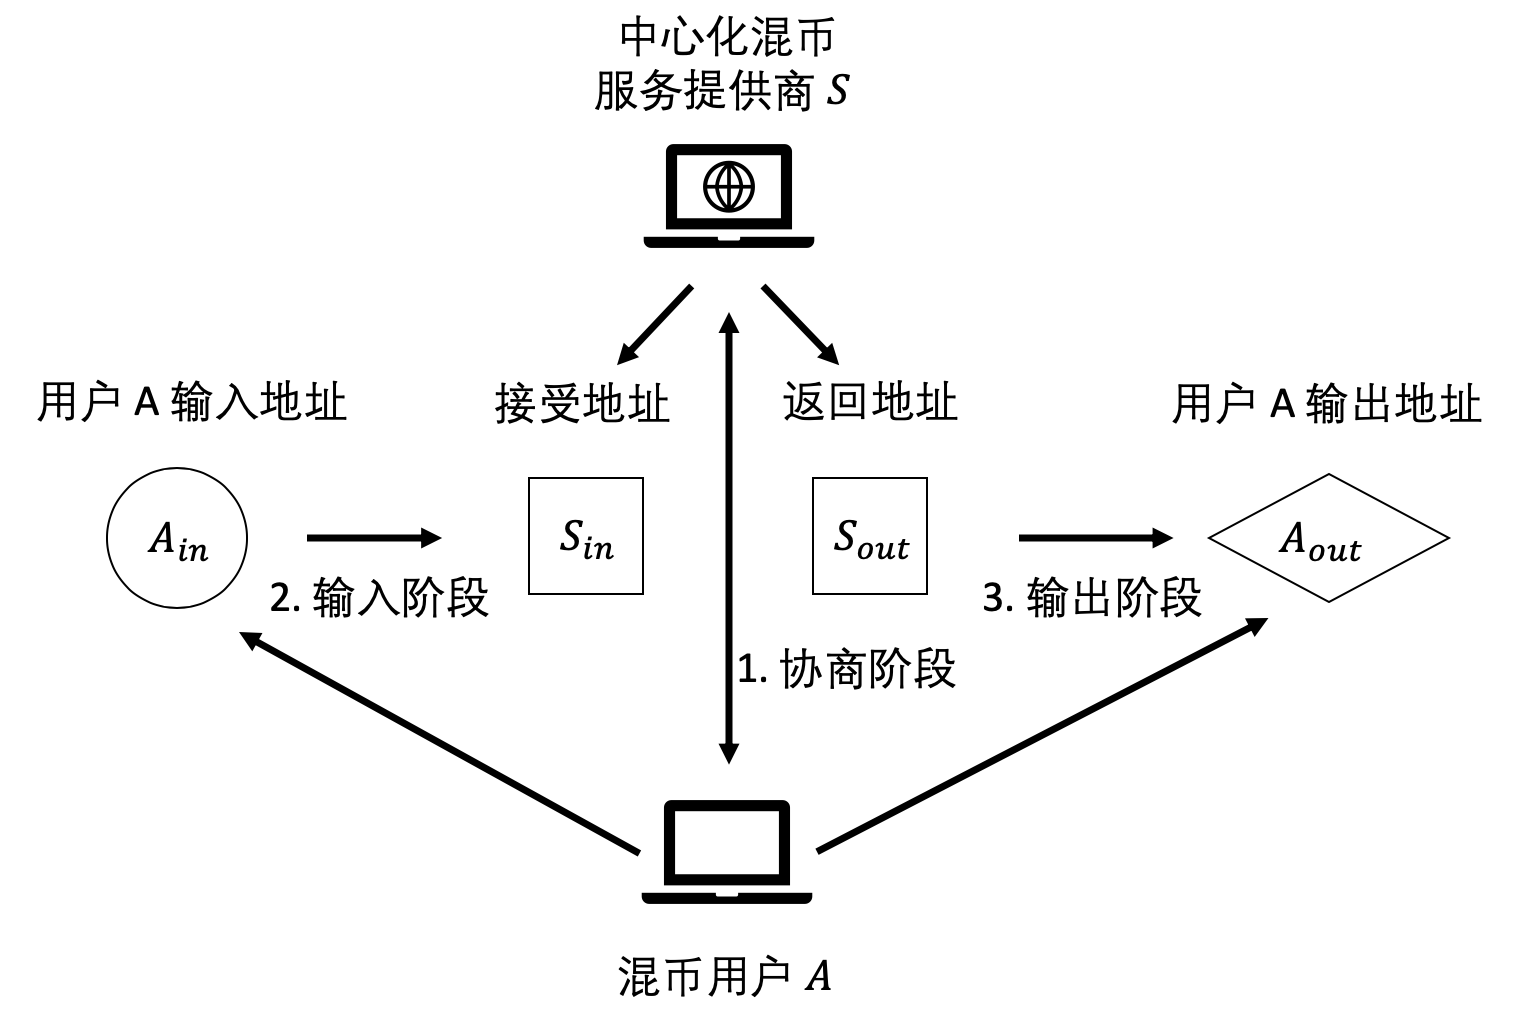
\includegraphics[height=7cm]{figures/cen-mixer.png}
\caption{中心化混币模型}
\label{fig:cen-mixer}
\end{figure}

中心化混币协议的基本模型如图\ref{fig:cen-mixer}所示,具体的协议流程主要分为协商、输入、输出及结束四个阶段:

\begin{enumerate}
	\item \textbf{协商阶段}:希望参与混币的用户与混币服务提供商进行协商,约定用户用于混币的输入地址、输出地址、服务提供商的接受地址、返回地址、混币金额、混币输入输出时间、混币手续费等相关参数。
	\item \textbf{输入阶段}:用户按照协商阶段商定的相关参数在约定时间之前将约定资产从输入地址发送到服务提供商指定的接受地址。
	\item \textbf{输出阶段}:服务提供商在约定时间之前将扣除手续费后的资产通过返回地址发送到用户指定的输出地址。
	\item \textbf{结束阶段}:若协议正常运行结束,服务提供商和用户销毁协商阶段留下的记录,保护用户隐私。
\end{enumerate}

最早的中心化混币服务例如BitLaundry平台采用最基础的中心化混币协议,用户将输入输出地址、交易金额以及交易时间等信息发送给BitLaundry,然后将对应金额的密码货币发送到BitLaundry指定的链上地址,BitLaundry确认接受后,将其他来源的对应数量货币返回到用户指定地址,并从中赚取固定手续费。这一方案的好处在于用户可以发送任意金额,并且指定交易的时间。然而BitLaundry平台的固定配置和暴露给用户的链上地址给攻击者提供了分析的机会,攻击者可以根据搜集的BitLaundry平台地址以及固定的手续费特征将混币交易提取并且关联在一起[38]。基础的中心化混币服务主要存在如下问题:

\begin{enumerate}
	\item 中心化混币服务提供商的行为存在一定特征,例如混币交易在时间上的规律,抽取一定比率的手续费,存在一个常用的地址池等等。攻击者可以通过上述特征进行混币交易的分析,将用户的输入输出地址关联起来,难以满足外部隐私性。
	\item 中心化混币服务提供商存在内部作恶的风险,无法保证在接受到用户输入资产后将对应资产返还给用户。在区块链系统中,所有链上地址都是算法生成的假名,因此用户无法证明自己的资产是否被窃取,平台也难以提供证据自证清白。此外,服务提供商也无法保证删除了用户输入输出关联关系的记录,因此不能满足资产安全性和内部隐私性。
\end{enumerate}
	
针对上述问题,研究者们提出了增加中心化混币协议外部隐私性、内部隐私性和资产安全性的相应技术。主要通过随机化机制减少混币服务提供商存在的特定行为特征,增加攻击者进行分析的难度,从而增强外部隐私性;通过要求混币服务提供商对协商阶段的参数进行数字签名作为承诺,以防服务提供商盗窃用户资产,增强资产安全性;通过在协商阶段使用盲签名技术,在保持承诺机制的前提下保护关键参数不对服务提供商可见,从而对服务提供商隐藏用户输入输出地址之间的关联关系,提供内部隐私性。

\subsubsection{随机化机制}

为了防止攻击者根据平台固定的手续费等配置来关联混币用户的输入输出地址,随机化机制通过中心化混币服务提供商在输出阶段人为制造交易时间、手续费等信息的随机性,掩盖混币交易的特征。中心化混币平台Bitcoin Fog将收取的手续费设定为一个范围之间的随机值,并在用户指定时间区间内随机挑选时间将资产返还到用户指定地址。这一方案可以减少外部攻击者根据混币特征关联用户地址的可能,在一定程度上保护用户隐私。

在实际应用中,用户为了防止中心化混币服务商泄漏用户隐私,会将资产在多家混币服务商依次进行混淆,此时连续的混币交易存在的手续费特征会暴露用户隐私。为解决这一问题,Mixcoin协议[15]设计了随机的、全有或全无(all-or-nothing)的手续费机制,混币服务提供商以约定好的概率将部分用户的混币金额全部留做手续费,其他用户的混币金额全额返还。为了保证生成随机数的可信性,Mixcoin采用约定区块链某未来区块的数据作为随机化参数,一定程度上保障随机数的不可伪造性。服务商M根据用户提供的参数 , , ,计算随机值 ,其中 表示第 个区块的交易二叉树根的值,PRNG为密码学伪随机数生成算法,根据输入参数生成(0,1)区间中对应的随机数。如果生成的随机值小于阈值,即 ,则服务商M收取所有混币资产作为手续费,否则返回全部资产。

采用随机化机制主要增强中心化混币方案的外部隐私性,防止外部攻击者通过混币交易存在的固定特征分析用户的混币过程。但不能提供内部隐私性与资产安全性,混币服务商可能盗窃用户资产或者泄漏用户地址关联关系等隐私信息。

\subsubsection{基于数字签名的承诺机制}

由于在区块链系统中,中心化的混币服务商没有实体身份作为信誉担保,可能出现盗窃用户资产的行为,用户很难相信混币服务商。同时用户的账户地址也不存在对应的身份,因而服务商难以自证清白。为了保护用户资产安全,混币服务商通过长期公钥代表身份建立承诺机制。在协商阶段,混币服务商需要提供身份对应的数字签名作为承诺。承诺包括约定的输入输出地址、混淆资产金额、约定时间等信息,并用混币服务商的长期公钥对应私钥进行签名。
	
利用数字签名技术提供不可伪造和不可抵赖的特性,增加承诺机制帮助用户证明平台的窃取行为。服务提供商通过维护自己的“虚拟声誉”,即代表身份的长期有效公钥,使得用户信任该服务商。使用该公钥对应私钥的签名向用户承诺平台不会出现盗窃行为,否则用户可以通过公开该承诺以及不符合承诺的区块链账本记录向其他用户证明该平台存在盗窃行为,破坏服务商的声誉。承诺机制一方面依靠在一定程度上保障了用户资产安全,另一方面也避免了用户恶意造谣。

\begin{figure}
\centering
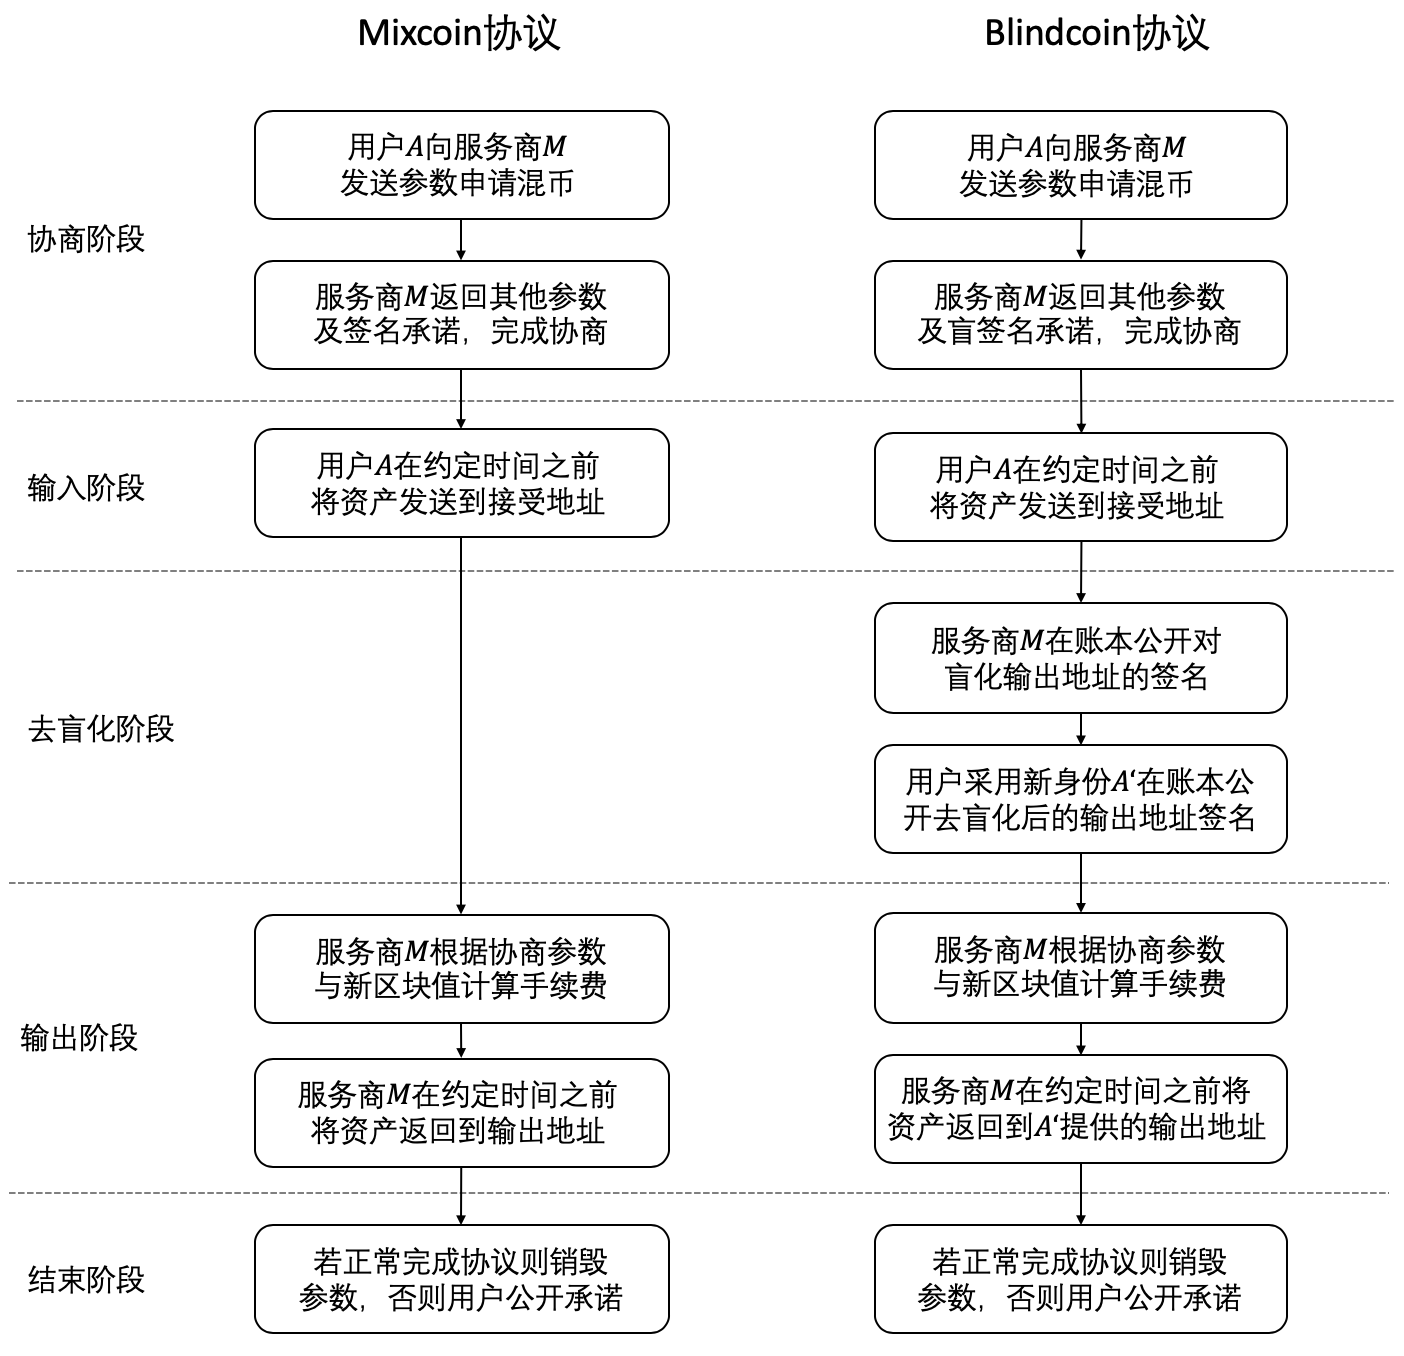
\includegraphics[width=10cm]{figures/mixcoin-blindcoin.png}
\caption{Mixcoin协议和Blindcoin协议}
\label{fig:mixcoin-blindcoin}
\end{figure}

2014年,Joseph等人提出了Mixcoin协议[15],通过基于数字签名的承诺机制增强资产安全性Mixcoin协议的核心步骤如图\ref{fig:mixcoin-blindcoin}所示,在协商阶段加入承诺机制,服务提供商需要对协商参数进行签名作为承诺,用户得到承诺后再向服务提供商支付混币资产。若服务提供商未按照承诺在约定时间之前返回资产,则用户在结束阶段可以公示在协商阶段收到的承诺与区块链账本记录的事实证明该服务提供商违背承诺。
	
Mixcoin协议通过承诺机制在一定程度上保护了用户的资产安全,但是该协议无法提供内部隐私性,即平台无法证明已如约销毁用户混币记录,用户也无法进行验证。因此用户为了保护自己的混币隐私不被恶意平台泄漏,通常采用在多个平台连续混币的方式。但这带来了较高的手续费,也留下更多的混币交易记录,给攻击者提供了更多特征进行分析。

\subsubsection{基于盲签名技术的隐藏机制}
为了提供中心化混币方案的内部隐私性,需要服务提供商在不知道用户输入输出地址对应关系的情况下进行输入和输出阶段,利用盲签名技术可以达到这一目的。1983年,Chaum等人[39]提出了盲签名的概念,盲签名技术是一种特殊的数字签名技术,在签名者对消息内容进行签名的过程中并不知道消息内容。盲签名技术满足以下两条性质,其中第一条特征保证了签名消息的内容隐私性,第二条特征保证了签名请求者的身份隐私性:
\begin{enumerate}
	\item 被签名消息对签名者是不可见的,即签名者不知道他所签署消息的具体内容。
	\item 签名消息不可追踪,即当签名消息被去盲化公布后,签名者无法将去盲化签名与盲化签名对应上。
\end{enumerate}

\begin{figure}
\centering
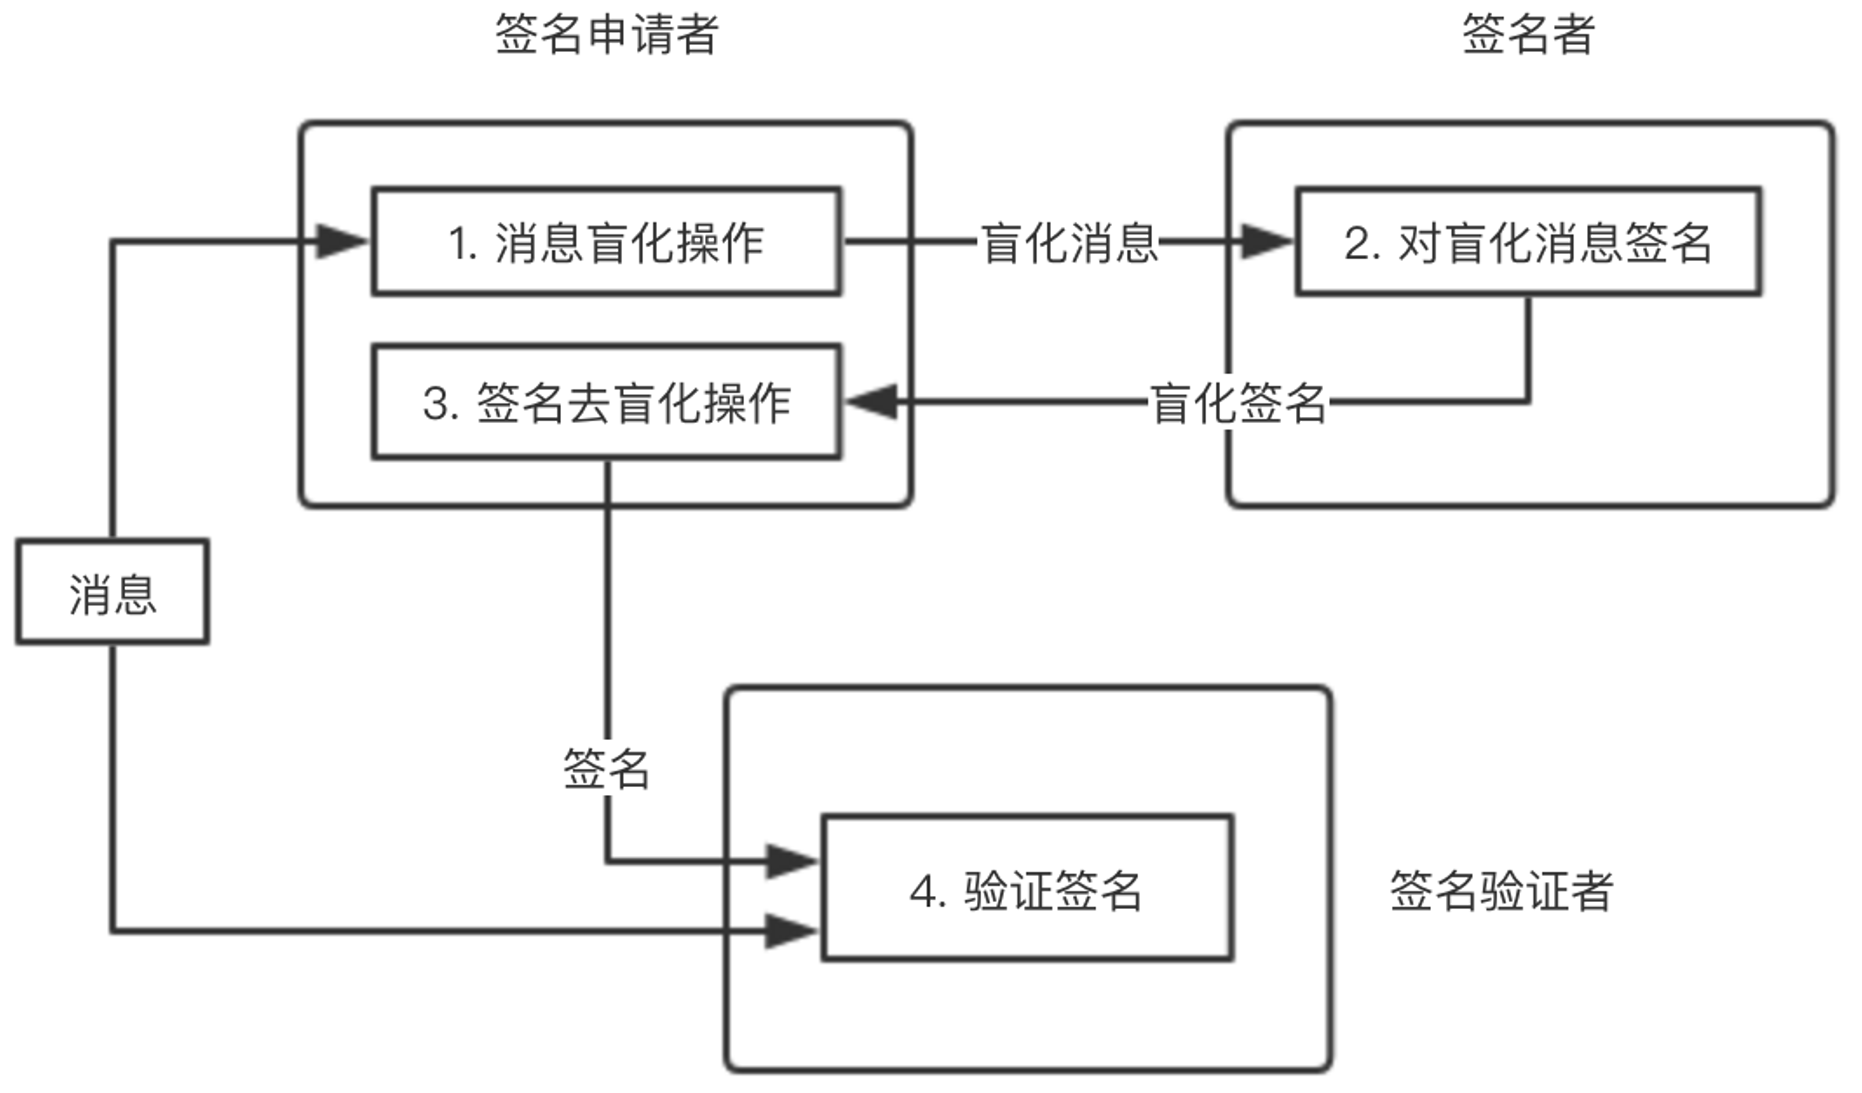
\includegraphics[width=10cm]{figures/blind-sig.png}
\caption{盲签名流程}
\label{fig:blind-sig}
\end{figure}

盲签名技术的整体流程如图\ref{fig:blind-sig}所示,主要分为以下四个步骤:

\begin{enumerate}
	\item 签名申请者首先将消息进行盲化操作,将盲化消息发给签名者。
	\item 签名者对盲化消息进行签名操作,将盲化签名返回签名申请者。
	\item 签名申请者对收到的盲化签名再作去盲变换,得出的便是签名者对原数据的签名。
	\item 签名申请者可以公布原始消息与去盲化签名,由验证者进行验证。
\end{enumerate}

2015年,Luke等人提出了Blindcoin协议[16],通过采用盲签名技术保障中心化混币方案的内部隐私性,核心步骤如图\ref{fig:mixcoin-blindcoin}所示。该协议保留了Mixcoin协议的随机化手续费、承诺等机制,并在此基础之上通过盲签名技术使得混币用户的输入输出地址关联关系对服务提供商不可见。该协议首先修改了协商阶段的签名部分,服务提供商对包含盲化的用户输出地址的承诺进行盲签名,然后用户对盲化签名进行去盲化操作得到针对真实输出地址的签名,并作为输出地址获取混币资产的凭证提交给服务商,服务商可以验证该签名的正确性以及是否使用过。由于服务商在协商阶段知道用户的输入地址但不知道输出地址,而在输出阶段知道输出地址而不知道对应的输入地址,因而无法判断用户输入输出地址的关系。盲签名技术可以有效增强中心化混币方案的内部隐私性,为了同时保持MixCoin方案中的可审计特性,该协议需要通过在公开的可信账本(论文推荐使用同一区块链)中记录下盲签名和去盲签名的内容,达到时间戳认证的效果。这一设计不会暴露用户的隐私,而一旦混币服务提供商未履行承诺,用户可以公示服务商提供的承诺,并使用在区块链账本中存储的消息作为违约证据。

\subsection{去中心化混币}

尽管中心化混币技术中系列协议在一定程度上保障了资产安全性和隐私性,但其依赖的混币服务提供商仍会带来一些潜在风险,例如遭受黑客攻击进而盗窃用户资产。研究者提出了一系列去中心化的混币协议,通过多方参与的协议代替中心化混币服务提供商,使得用户不需要先将自己的比特币发送给混币服务提供商,而是在网络中找到其他需要混币的用户,通过多方参与者运行协议的方式构造一致的混币交易,确认后签名使得交易生效。这一系列协议从根本上解决了中心化混币存在的信任问题,同时节省了混币服务提供商收取的手续费。但是也存在着一些不足,比如寻找其他混币用户存在困难,容易让外部攻击者混入并监听混币关系甚至进行拒绝服务攻击(DOS,Denial of Service)导致混币失败。
 
\begin{figure}
\centering
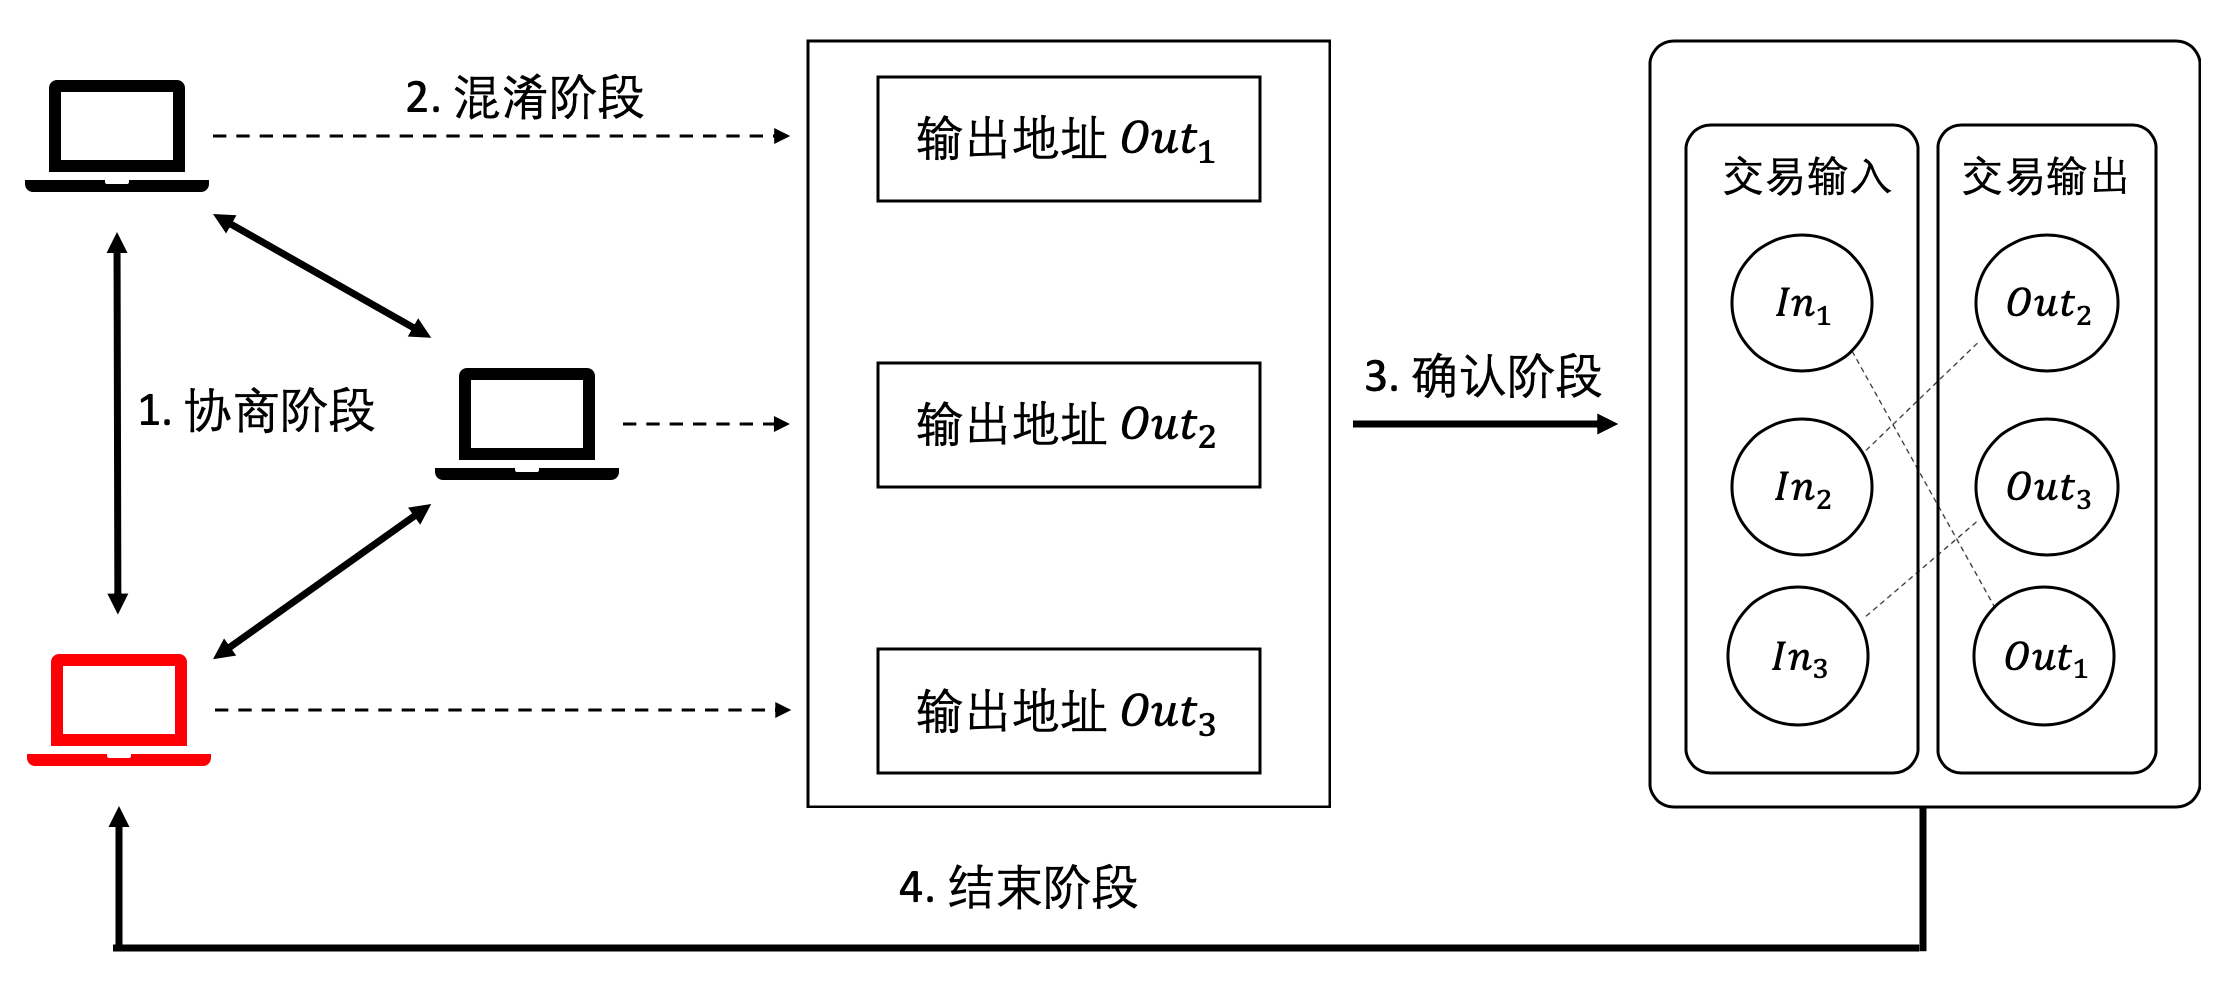
\includegraphics[width=10cm]{figures/decen-mixer.png}
\caption{去中心化混币模型}
\label{fig:decen-mixer}
\end{figure}

去中心化混币协议的基本模型如图\ref{fig:decen-mixer}所示,分为协商、混淆、确认及结束四个阶段,其中红色节点表示混入的攻击者。与中心化混币协议的区别主要在于执行的角色由中心化混币服务器转变为参与混币的用户多方共同完成:

\begin{enumerate}
	\item 协商阶段:用户寻找参与混币的其他同伴,协商去中心化混币协议需要的参数,例如各用户混币输入输出地址、混币金额等参数。
	\item 混淆阶段:参与混币的用户根据协议对所有输出地址进行混淆,隐藏用户输入输出地址之间的关联关系。
	\item 确认阶段:混币用户根据混淆阶段得到混淆后的交易输出,构造混币交易,确定无误后进行广播,将混币资产发送到各用户指定的输出地址。
	\item 结束阶段:若混币协议正常结束,参与混币的各用户销毁此次混币过程相关记录,若过程出现错误中止,参与混币的用户找出并且排除造成错误的用户。
\end{enumerate}

去中心化混币技术根据参与方的数量主要分为多方混币技术与双方混币技术两类。其中多方混币技术参与者数量大于等于3,且隐私保护程度与参与者数量成正相关。其优点在于多参与方增强了地址混淆的外部隐私性,多参与方构造一笔交易也能节省交易费。缺点在于参与者数量的上升会增大攻击者混入的概率,攻击者可以在协议过程中监听并分析其他参与者的输入输出地址关联关系,威胁内部隐私性,甚至进行拒绝服务攻击中断协议进程。双方混币技术只有两个参与方,单次混淆只能提供一定的外部隐私性,并且不能提供内部隐私性,因此双方混币技术中用户需要与不同参与方进行多轮混币来增强隐私性。优点在于提升了协议的隐私性,并且每次的混币操作简单,缺陷在于多次混币需要进行多次交易,带来了高额交易费。

\subsubsection{多方混币技术}
多方混币技术主要模型为n个参与方约定相等的混币金额,构建n-to-n的多签名交易,保证每个交易输出都为相等的金额,外部攻击者无法通过分析该交易分辨不同的输出,从而无法分析每个输出与输入地址之间的关联关系,保障外部隐私性。

\begin{figure}
\centering
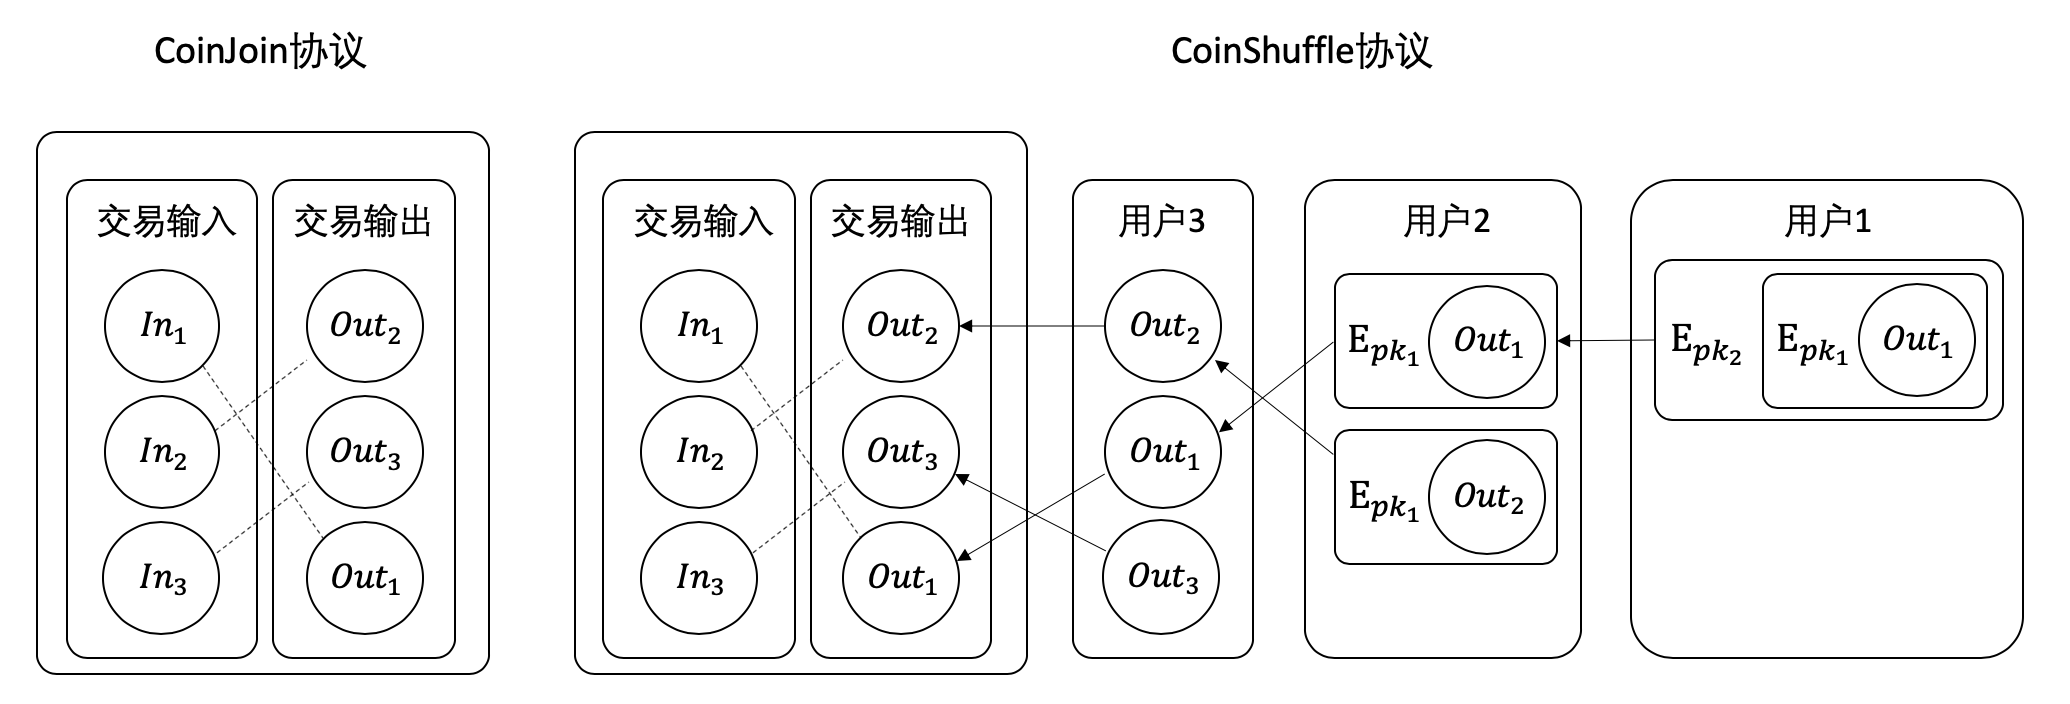
\includegraphics[width=10cm]{figures/coinjoin-shuffle.png}
\caption{CoinJoin协议和CoinShuffle协议}
\label{fig:coinjoin-shuffle}
\end{figure}

2013年8月,Gmaxwall提出了CoinJoin协议[17],如图\ref{fig:coinjoin-shuffle}所示,该协议在协商阶段由参与混币的用户协商输入输出地址、统一输出金额等参数,然后在混淆阶段将所有输入和输出放入同一交易中构造混币交易,确认阶段中,各参与者检查自己的输出无误后对输入进行签名,当所有参与用户完成签名后将该交易广播到网络中。这一协议操作十分简单,参与用户无需信任其他节点,也不用缴纳混币手续费,攻击者无法分辨n个金额一致的输出资产,保障协议的外部隐私性。并且用户可以先检查混币交易中自己的输出地址与金额是否正确,然后决定是否对交易输入进行签名,提供了资产安全性。但是,CoinJoin协议的缺陷在于协商阶段中参与用户的输入输出地址关联信息会被其他参与混币的用户获取,不能提供地址混淆的内部隐私性。此外,一旦参与混币的部分节点拒绝签名或者提前花费参与混币的输入资产,会导致混币失败。因此内部隐私性不能得到保障。

基于CoinJoin协议的Dash项目[3]在此基础上进行一定的改进,该项目中的混币交易由网络中的主节点构造保证了内部隐私性。多个主节点为用户的交易进行链式混币,上一个主节点的交易输出作为下一个主节点的交易输入进一步混淆,为了便于不同金额的交易进行,Dash将所有金额拆分为十进制单位的和。由于每次混淆交易要求至少3位参与者,因此随着混淆链的增长,混淆集合的用户数量呈指数上升,极大增强混淆能力。也保证了只要攻击者不能控制混淆链中大部分的主节点,就难以判断用户的输入输出地址的对应关系。

除了Dash中引入主节点的方案外,为了解决CoinJoin方案中的地址关联关系泄漏问题,保障地址混淆的内部隐私性。2014年,Tim等人提出了去中心化混币协议CoinShuffle[18],该协议继承了CoinJoin的思想,使得多个混币参与者共同发起同一输出金额的交易,并且参与者可以检查交易后再签名以确保资产安全性。此外,该协议借鉴了可审计的匿名群组消息传递协议Dissent[40],采用多层加密隐藏输入输出地址的关联关系,提供内部隐私性。如图\ref{fig:coinjoin-shuffle}所示,在混淆阶段中,各用户按照一定顺序进行排列,用户1将自己输出地址通过用户n到用户2的公钥依次进行加密,得到多层加密结果,然后发送给用户2。各用户将接受到的地址集合中各地址用私钥进行解密,然后加入自己多层加密后的输出地址,发送到下一个用户。最后用户n解密得到其他所有用户的输出地址并加入自己输出地址进行混淆。混淆过程中,除了用户n以外的用户不能得知其他用户的输出地址明文,而用户n也无法得知其他用户与输出地址的对应关系,保障了内部隐私性。CoinShuffle协议的优点在于通过多层加密提供了内部隐私性,同时也继承了CoinJoin的外部隐私性和资产安全性。缺陷在于该方案的混淆阶段计算量较大,花费时间较长,并且需要所有用户同时在线。尽管设计了问责阶段发现进行错误行为的参与者,但也可能遭受攻击者的拒绝服务攻击,一旦遭受拒绝服务攻击则需要重新进行大量计算。此外,CoinShuffle协议构造的交易通常存在输出地址为输入地址两倍并且一半输出金额相等的特征,因此攻击者可以利用该特征找出CoinShuffle协议构造的交易并且将另一半找零地址与各输入地址关联[41]。

\begin{figure}
\centering
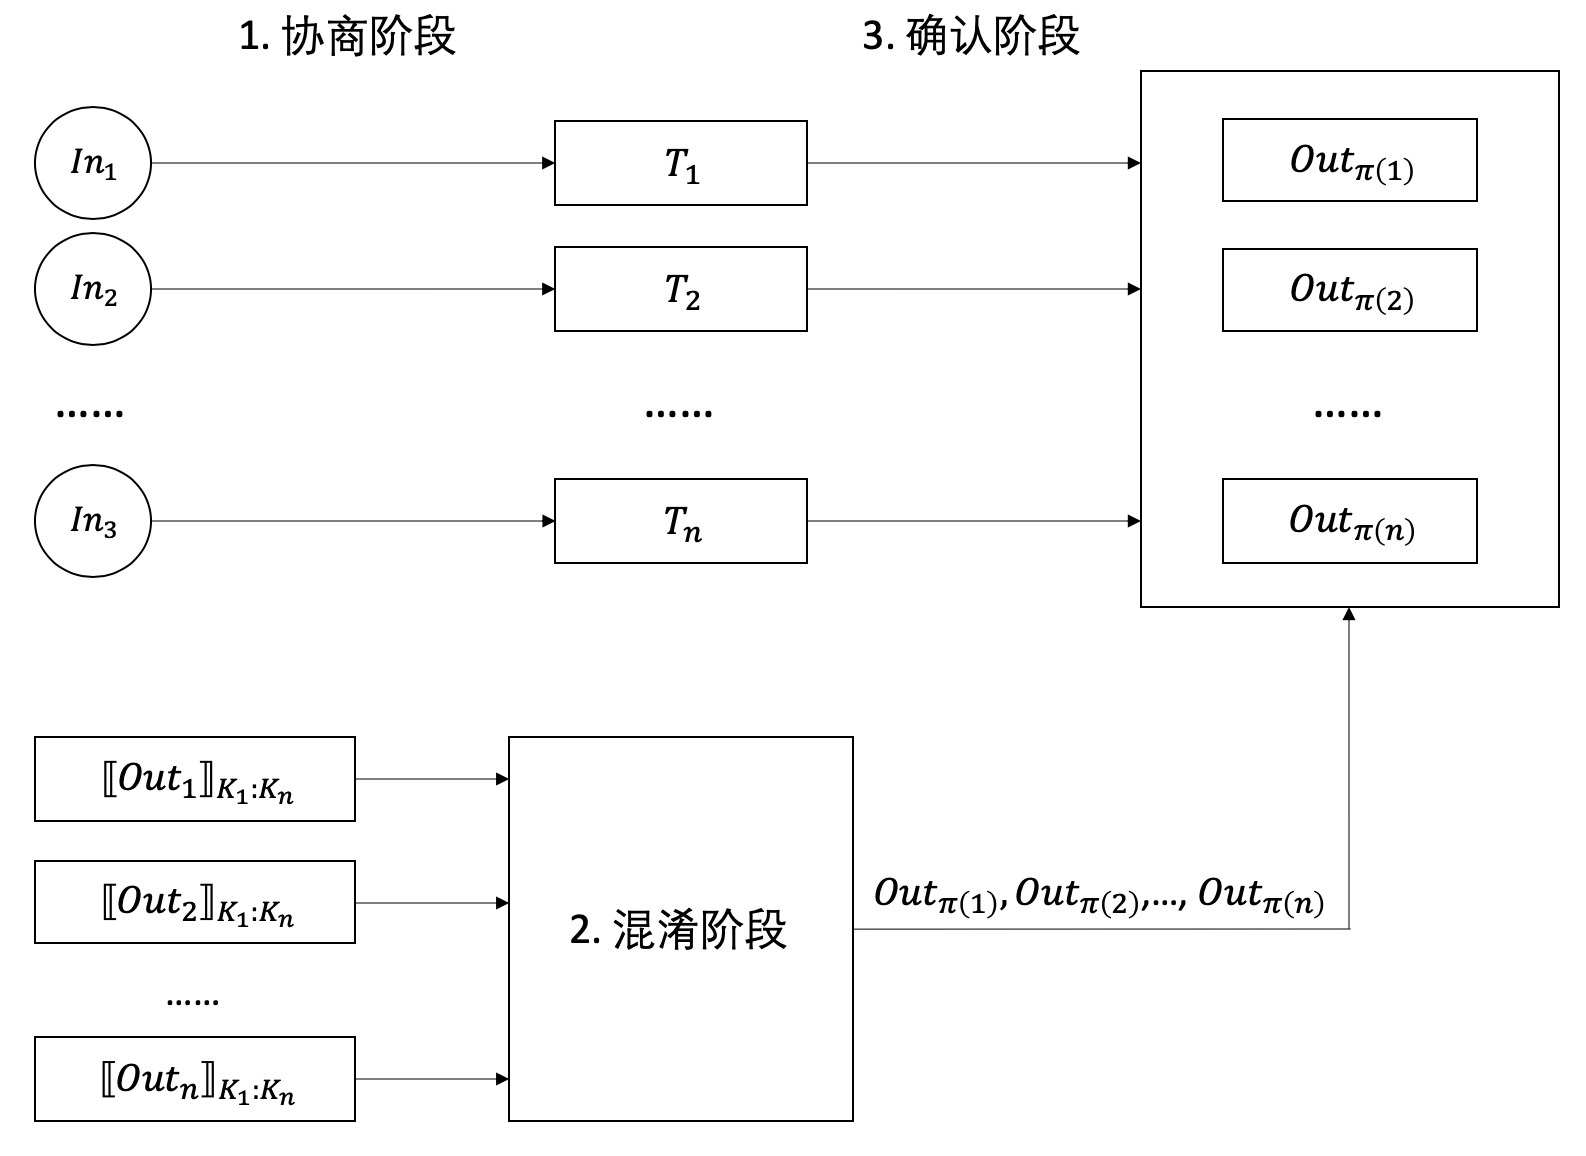
\includegraphics[width=10cm]{figures/coinparty.png}
\caption{CoinParty协议}
\label{fig:coinparty}
\end{figure}

为了解决CoinShuffle协议中混淆阶段遭受拒绝服务攻击损失较大的问题, 2015年,Jan等人提出基于安全多方计算技术的去中心化混币协议CoinParty[19],在协商阶段中,通过构建门限托管账户,接受参与者的输入资产作为抵押,增加了攻击者在混淆阶段进行拒绝服务攻击的成本。当攻击者数量较少时,正常参与的混币用户可以保障协议正常进行。CoinParty协议具体流程如图\ref{fig:coinparty}所示,在协商阶段各参与者将混币金额转入各自的临时托管地址作为抵押,表示承诺加入混币过程。临时托管地址由所有参与者通过伪随机秘密分享协议(PRSS,Pseudo-Random Secret Sharing)[42]共同生成,并需要大部分参与者共同签名才能使用,所以参与者无法独自取回抵押资产。完成协商后,CoinParty协议的混淆阶段将各参与者的输出地址进行混淆,与CoinShuffle协议同样采用了多层加密保障内部隐私性,但在CoinShuffle的基础上主要进行了两点改进,一方面采用秘密分享的校验和对比所有输出地址哈希值的和,对混淆结果进行校验;另一方面,CoinShuffle协议中最终的混淆结果由最后一位参与者决定而非随机决定,攻击者可以控制顺序。CoinParty协议以校验和作为伪随机数生成器的依据生成公共随机置换,要求最后一位参与者以字典序排序,再增加公共随机置换得到最终混淆结果,避免最后一位用户操纵排序结果。确认阶段中所有用户一同将各托管地址中存放的资产发送到混淆后对应的输出地址,即使少部分攻击者拒绝参与的情况下正常用户也能完成确认过程。

CoinParty协议的安全性保证在攻击者数量小于总参与者数量1⁄3的情况,但是在没有身份认证的情况下,攻击者可能进行女巫攻击[43],通过布置达到总参与者数量2⁄3的节点参与CoinParty协议,可以盗窃其他参与者的资产。因此该协议能提供内部隐私性和外部隐私性,但资产安全性存在一定风险。

\subsubsection{双方混币技术}

多方混币协议构造过程较为复杂,恶意攻击者加入后发布错误信息或中途退出会导致混币交易构造失败,因此容易受到拒绝服务攻击。而该类协议的隐私保护程度与混币交易参与者数量成线性正相关,为了增强外部隐私性希望加入更多参与者,但同时参与方越多也越容易引来恶意攻击者参与,给用户隐私以及混币成功率带来风险。为了防止恶意攻击者参与混币,研究者提出将单次混币操作限定在两个用户之间进行,降低恶意攻击者混入的概率,也减小攻击者攻击的危害。双方混币协议的核心思想在于将多个参与者进行一次混币交易改为混币用户多次寻找不同的混币同伴进行多轮双方混币,最终达到相同外部隐私性的混币效果。这类协议的优点在于攻击者为了获取用户资产流动,必须参与该用户的每一轮混币,但这概率上难以达到,从而减少了攻击者的威胁。缺陷在于多轮混币需要在区块链账本上发布多次交易,增加了交易费的支出,也带来了额外的时间花费。由于只有两个用户参与混淆,因此双方混币技术不存在混淆阶段。

2013年,Gmaxwall提出了CoinSwap协议[20],通过借助第三方用户作为中转隐藏交易直接输入方与直接输出方之间的关联。该协议通过第三方中间用户进行转账并保障资产安全。为了在无信任的情况下保障用户进行诚实的行为,协议中利用区块链系统中的哈希时间锁定合约(HTLC,Hashed Timelock Contract)保证参与各方的资产安全。哈希时间锁定合约包含哈希锁定与时间锁定,用户可以提供合约中哈希值的哈希原像作为私密值解锁资产,也可以在锁定时间之后使用地址签名解锁资产。哈希锁用于交易接收方接收资产,时间锁用于发起方在发生异常的情况下,一定时间后取回资产。
 
\begin{figure}
\centering
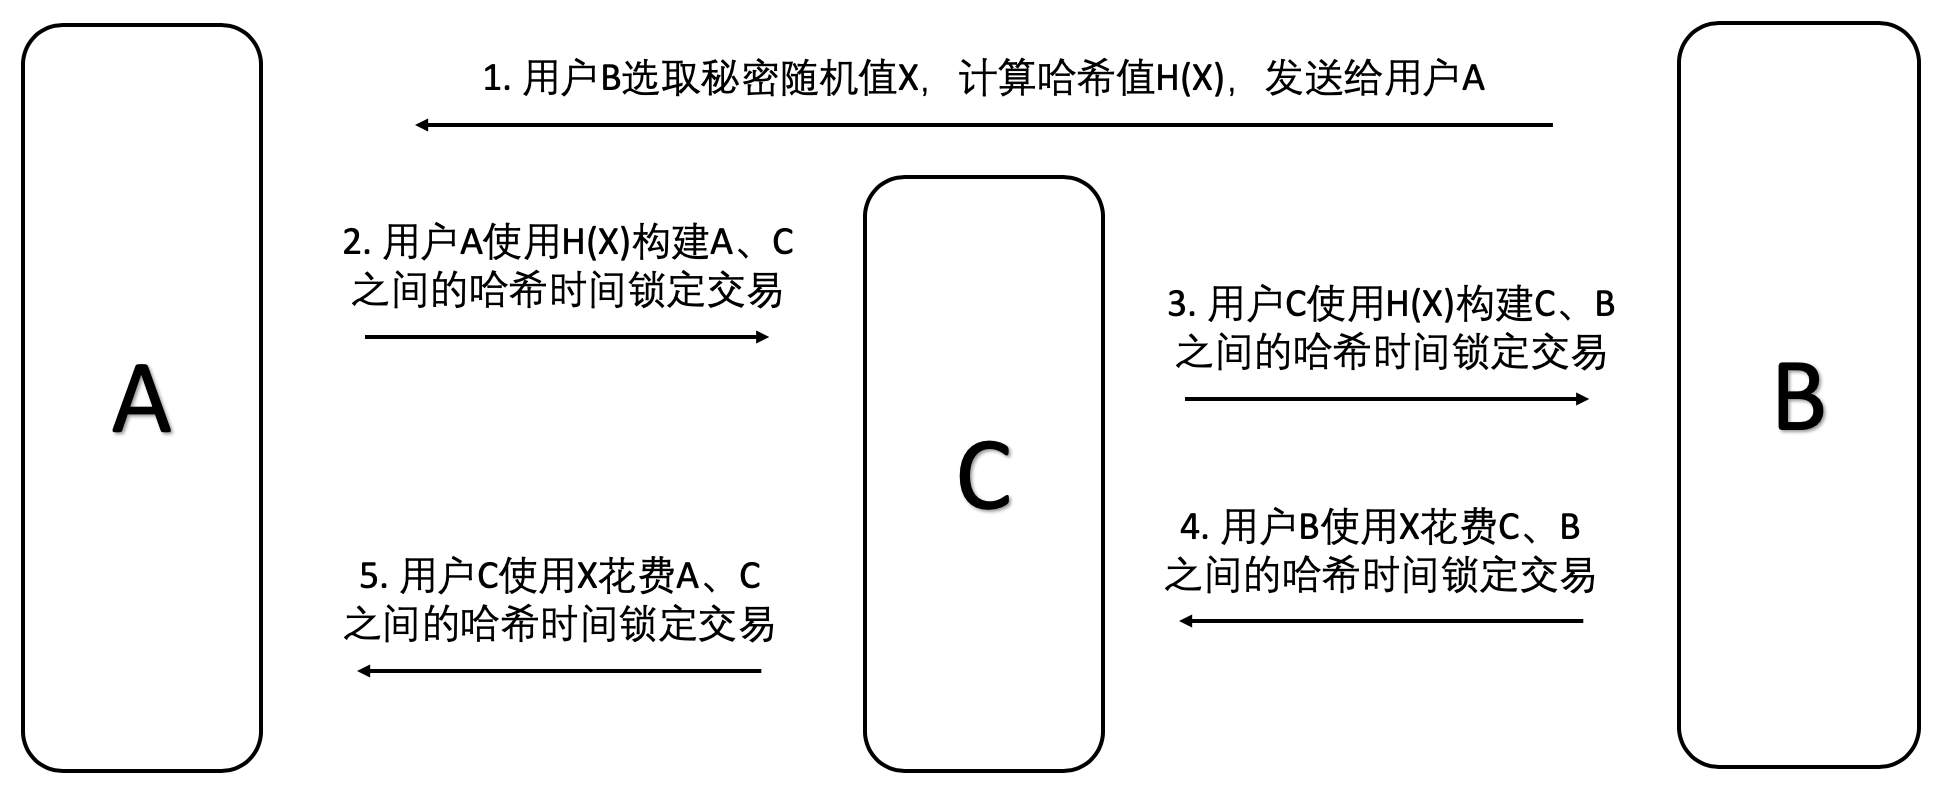
\includegraphics[width=10cm]{figures/coinswap.png}
\caption{CoinSwap协议}
\label{fig:coinswap}
\end{figure}

CoinSwap协议流程如图\ref{fig:coinswap}所示,混币交易并非构造在同一交易中,而是先由用户A向用户C发起交易,再由用户C向用户B发起交易。为了保证资产安全,该协议中的交易采用哈希-时间-签名锁,其中哈希锁利用用户B持有的私密值保证在用户B发布私密值获取资产后,用户C得知该私密值才能获取相应资产,签名锁保证用户B不能仅靠私密值获取用户A发给用户C的资产,同时采用时间锁保证在其他用户离线的情况下用户能取回自己的资产,防止拒绝服务攻击。由于用户A和用户B可以由同一用户扮演,因此该协议也可以用于双方混币。CoinSwap协议的优点在于通过哈希-时间-签名锁定合约能在无第三方参与的情况下完成混币,减少了攻击者参与的可能性,同时保障各参与用户的资产安全。缺陷在于至少多次交易带来的额外交易手续费以及两阶段交易构造与解锁带来的更长交易确认时间。

CoinSwap协议通过减少单次混币参与者数量,在一定程度上解决了攻击者监听和拒绝服务攻击的问题,但是仍存在一定隐私风险,攻击者可以通过女巫攻击的方式,尽可能多的布置混币节点,参与混币过程,攻击用户隐私安全。为了更进一步防止攻击者加入混币交易,2014年,George等人提出了能抵抗女巫攻击的去中心化混币协议Xim[21]。

Xim方案在协商阶段采用登记广告的方式构建同伴发现算法(见算法1),在公开的消息记录账本中发布广告与留言寻找混币同伴,需要支付一定的广告费,回应广告也需要支付一定手续费,用户从所有回应的用户中随机挑选同伴。因此,同时参与Xim混币的用户越多,攻击者为了让目标用户选择自己作为混币同伴,必须支付大量广告费,攻击代价随着参与Xim混币的用户数量线性增加,因而该协议能有效抵御女巫攻击。在混淆阶段,Xim协议中采用Barber等人提出的FairExchange协议[44]。Xim协议通过手续费机制提高攻击者进行女巫攻击及拒绝服务攻击的代价。此外,Xim协议的混淆范围包含当时参与Xim协议的所有参与者,极大提升了混币交易的外部隐私性。

综上所述,通过混淆账户地址保护用户隐私的机制有多种不同的技术实现。本文从协议中心化程度、资产安全性、隐私性、手续费等多个方面对介绍的协议进行了对比分析。如表3所示:

\section{信息隐藏机制}

地址混淆机制能在一定程度上保护账本隐私,但是地址混淆的结果仍会在公开账本中存储,攻击者可以通过分析带有特征的混淆交易一定程度上威胁用户隐私。为了增强隐私性,研究者们尝试将区块链账本中记录的信息包括交易发起者、交易接受者、交易金额等进行加密隐藏。另一方面,攻击者可以直接在区块链网络中监听节点信息以及通信情况,将链上内容与节点的真实情况关联,威胁用户网络隐私,可以通过隐藏网络节点信息和节点间流量来保护网络隐私。目前主要的信息隐藏技术主要隐藏以下几类隐私信息:

\begin{itemize}
	\item 交易发起者地址:区块链账本中交易的发起者地址信息,可以达到隐私保护不可追溯性,攻击者不能得到某交易发起的用户信息,保障发起者隐私。
	\item 交易接受者地址:区块链账本中交易的接受者地址信息,可以达到隐私保护不可关联性,攻击者不能将同一用户接受的两笔交易进行关联,保障接收者隐私。
	\item 交易金额:区块链账本中交易的具体金额信息。
	\item 网络节点信息:区块链网络中节点之间直接连接,需要隐藏消息发布节点的IP等信息。
	\item 网络节点间流量:区块链网络中节点间的信息流量情况,攻击者可以通过分析当前网络中流量攻击节点隐私,因此需要隐藏网络节点间流量。
\end{itemize}

信息隐藏机制的主要优点在于采用密码学加密技术提供了较高的数据隐私安全性。此外,相较于地址混淆机制,用户不需要寻找其他混淆用户进行合作。缺陷在于更大的计算量和存储空间要求。根据隐藏信息的内容,主要可以分为账本信息隐藏技术和网络数据隐藏技术,其中账本信息隐藏技术针对保护区块链账本中记录的信息包括交易发起者地址、接受者地址以及交易金额,保护账本隐私信息。而网络数据隐藏技术主要针对保护区块链网络中的节点信息以及节点间流量,保护网络隐私信息。

\subsection{账本信息隐藏}

账本信息隐藏主要防范区块链账本公开带来的账本分析攻击,通过对账本中隐私数据进行加密,保护账本隐私。并且通过密码学技术提供“凭证”,保持区块链账本正确性的可验证。现有的账本信息隐藏机制的实现技术大多属于零知识证明技术[45],零知识证明即除了所讨论命题的正确性之外不传达任何其他知识的证明。零知识证明协议中存在两种角色:证明者和验证者,证明者向验证者提供证据证明某命题成立,但不泄露除结论外的其他任何信息,验证者需要验证该证明的正确性。因此零知识证明协议需要满足三个重要属性:

\begin{enumerate}
	\item 完整性:如果证明者能证明命题成立,那么他能提供证明说服验证者。
	\item 可靠性:如果证明者不能证明该命题成立,那么他不能伪造证明欺骗验证者。
	\item 零知识性:在验证者验证证明的过程中,不能得到除了命题正确性以外的任何信息。
\end{enumerate}

相关研究者提出了许多具体零知识证明方案。例如哈密顿回路[46]和三着色问题的零知识证明方案[47]等。具体的解决方案根据应用场景不同各有差异,可以根据证明者和验证者是否需要交互分为“交互式零知识证明”(IZK, Interactive Zero-Knowledge Proof)和“非交互式零知识证明”(NIZK,Non-Interactive Zero-Knowledge Proof)[48]两类。目前在区块链领域中应用非交互式零知识证明技术,证明者可以随时独自构造并发起交易。

账本数据隐藏技术的主要衡量指标包括以下几点:

\begin{itemize}
	\item 隐藏内容:隐藏账本中的隐私数据,主要包括交易发起地址、接受地址、金额等内容。通常账本数据隐藏技术能保护其中一类内容,区块链系统通过同时采用多种技术保护多类隐私数据。
	\item 计算复杂度:构建交易和验证交易正确性的计算复杂度。由于采用了较为复杂的密码学技术进行加密和验证,因此账本数据隐藏技术给交易的构造和验证都带来了较大的计算复杂度。
	\item 空间复杂度:交易在区块链账本中占据的空间大小。采用账本数据隐藏技术构建的交易,为了证明正确性需要附带凭证,比直接保存原始数据带来更大的空间开销。
\end{itemize}

\subsubsection{密码累加器技术}

为了判断一个数据是否在某一集合中,传统的解决方案包括逐个比较,二分法查找等,这些算法的时间复杂度和空间复杂度都随着集合的增大而增加。为了解决这一问题,1993年,Benaloh等人[49]提出了“累加器”的概念,通过将整个集合组合到一个较小的累加器数据中,达到以固定大小的证据证明某元素在累加器中的效果。然而这一累加器不能从中删除元素。为了解决这一问题,2002年,Camenisch等人[50]提出了“动态累加器”的概念,基于非对称加密体系RSA[51]构造了能动态增删元素的累加器。同时,为了让用户在证明累加器中某元素存在性的同时不暴露具体元素,该研究构造了动态累加器的零知识证明。 
 
\begin{figure}
\centering
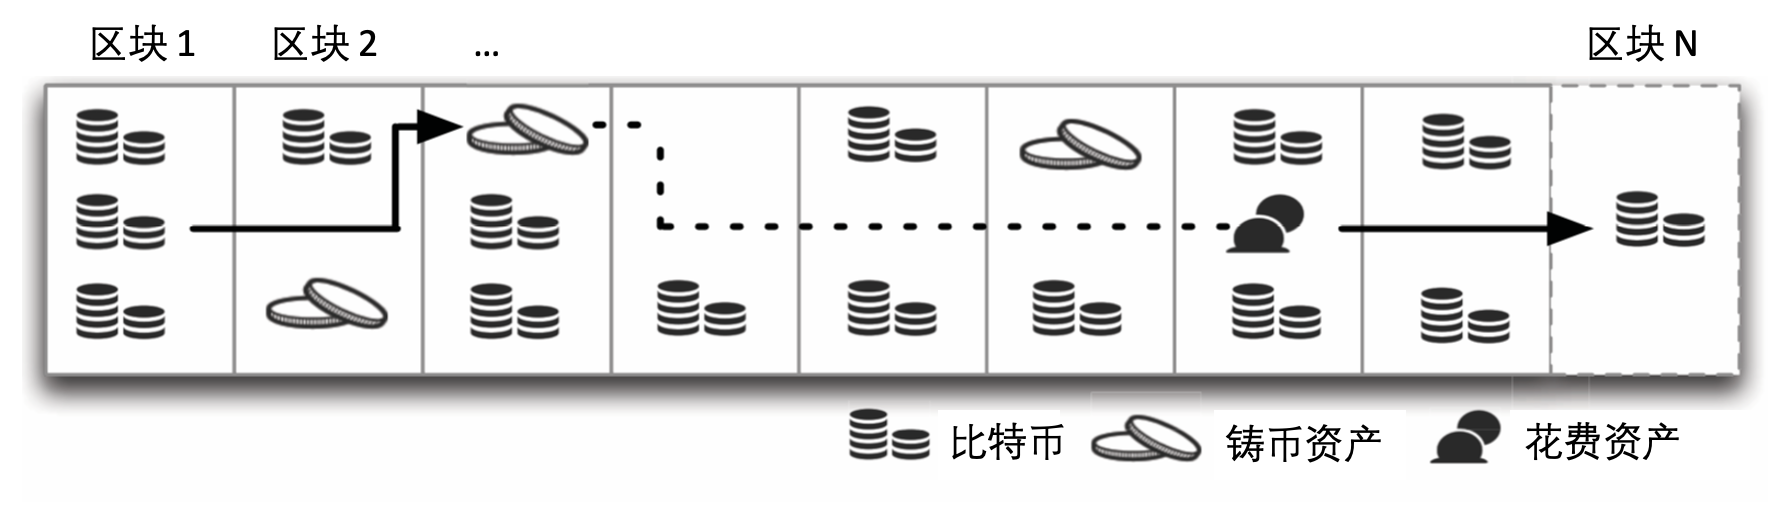
\includegraphics[width=10cm]{figures/zerocoin.png}
\caption{ZeroCoin账本示意图}
\label{fig:zerocoin}
\end{figure}

为了抵抗区块链账本公开带来的账本分析攻击,2013年,Miers等人基于比特币系统提出了ZeroCoin协议[22],这一协议如图\ref{fig:zerocoin}所示,用户可以独自进行混币操作,通过铸币交易将资产加入密码累加器,生成私密资产,达到和所有使用ZeroCoin的用户共同混币的效果。当用户需要使用之前加入累加器的资产时,根据参数生成凭证,证明自己拥有累加器资产集合中的某一未曾花费过的资产,花费该资产生成等额比特币。ZeroCoin的优点在于节点可以通过验证花费资产是否存在累加器中以及是否使用过来验证交易是否合法,但不能将用户使用的资产和此前的铸币交易对应,这样用户就完成了和整个资产集合的混淆,攻击者无法分析该资产的关联关系。并且用户可以独立完成混币交易的构造,不需要依赖任何混币服务提供商,也不需要寻找其他混币用户。攻击者无法根据用户生成的参数关联用户的铸币地址和花费地址。然而,ZeroCoin的缺点主要有三点:第一点是计算资源和交易体积的增加,这导致区块链账本的交易容量更小,也导致区块链系统性能下降;第二点是算法的初始全局参数需要可信第三方来生成,但这在公有链系统中很难得到用户的信任;第三点是无法隐藏交易金额,因此为了保护隐私,规定所有铸币和花费操作都只能使用固定值的资产,实际使用中并不方便。

\subsubsection{零知识证明技术}

简明非交互式零知识证明(zk-SNARK,zero-knowledge Succinct Non-interactive ARguments of Knowledge)技术在非交互式零知识证明证明技术的基础之上进行优化,保持非交互性的同时,减少了证明大小,节省存储空间与验证时间。该技术主要应用于可验证计算领域。zk-SNARKs技术主要由密钥生成算法、证明生成算法和证明验证算法组成。其中密钥生成算法由初始化参数生成证明密钥pk和验证密钥vk;证明生成使用证明密钥pk生成对声明x和证据a的证明 π;证明验证算法使用验证密钥验证声明x的证明 π 是否正确。该技术满足以下特征:

\begin{itemize}
	\item 完备性:对任意正确的声明x,持有证据a的证明者能生成正确的证明 π,使验证者验证其正确性。
	\item 简明性:正确生成的证明 π 空间复杂度为常数,证明验证算法的时间复杂度仅与声明x的长度成线性相关。
	\item 不可伪造性:不知道证据a的证明者无法生成正确的证明 π。
	\item 完美零知识性:验证者除了判断声明x正确性以外不能获取任何信息。
\end{itemize}

2013年,Parno等人[52]提出实现zk-SNARKs的Pinocchio 系统,该系统先将计算拆分为一阶线性约束等式(R1CS, Rank-1 Constraint System),然后转换为多项式运算形式(QAP,Quadratic Arithmetic Programs),将计算的验证转换为对多项式等式的验证,通过对点的抽样计算完成对整个多项式等式正确性的检验,基于椭圆曲线的双线性对性质隐藏用于计算的真实输入,利用可信创始方初始化阶段生成的参数实现零知识证明。该实现的安全性依赖于QAP问题的不可计算。

\begin{figure}
\centering
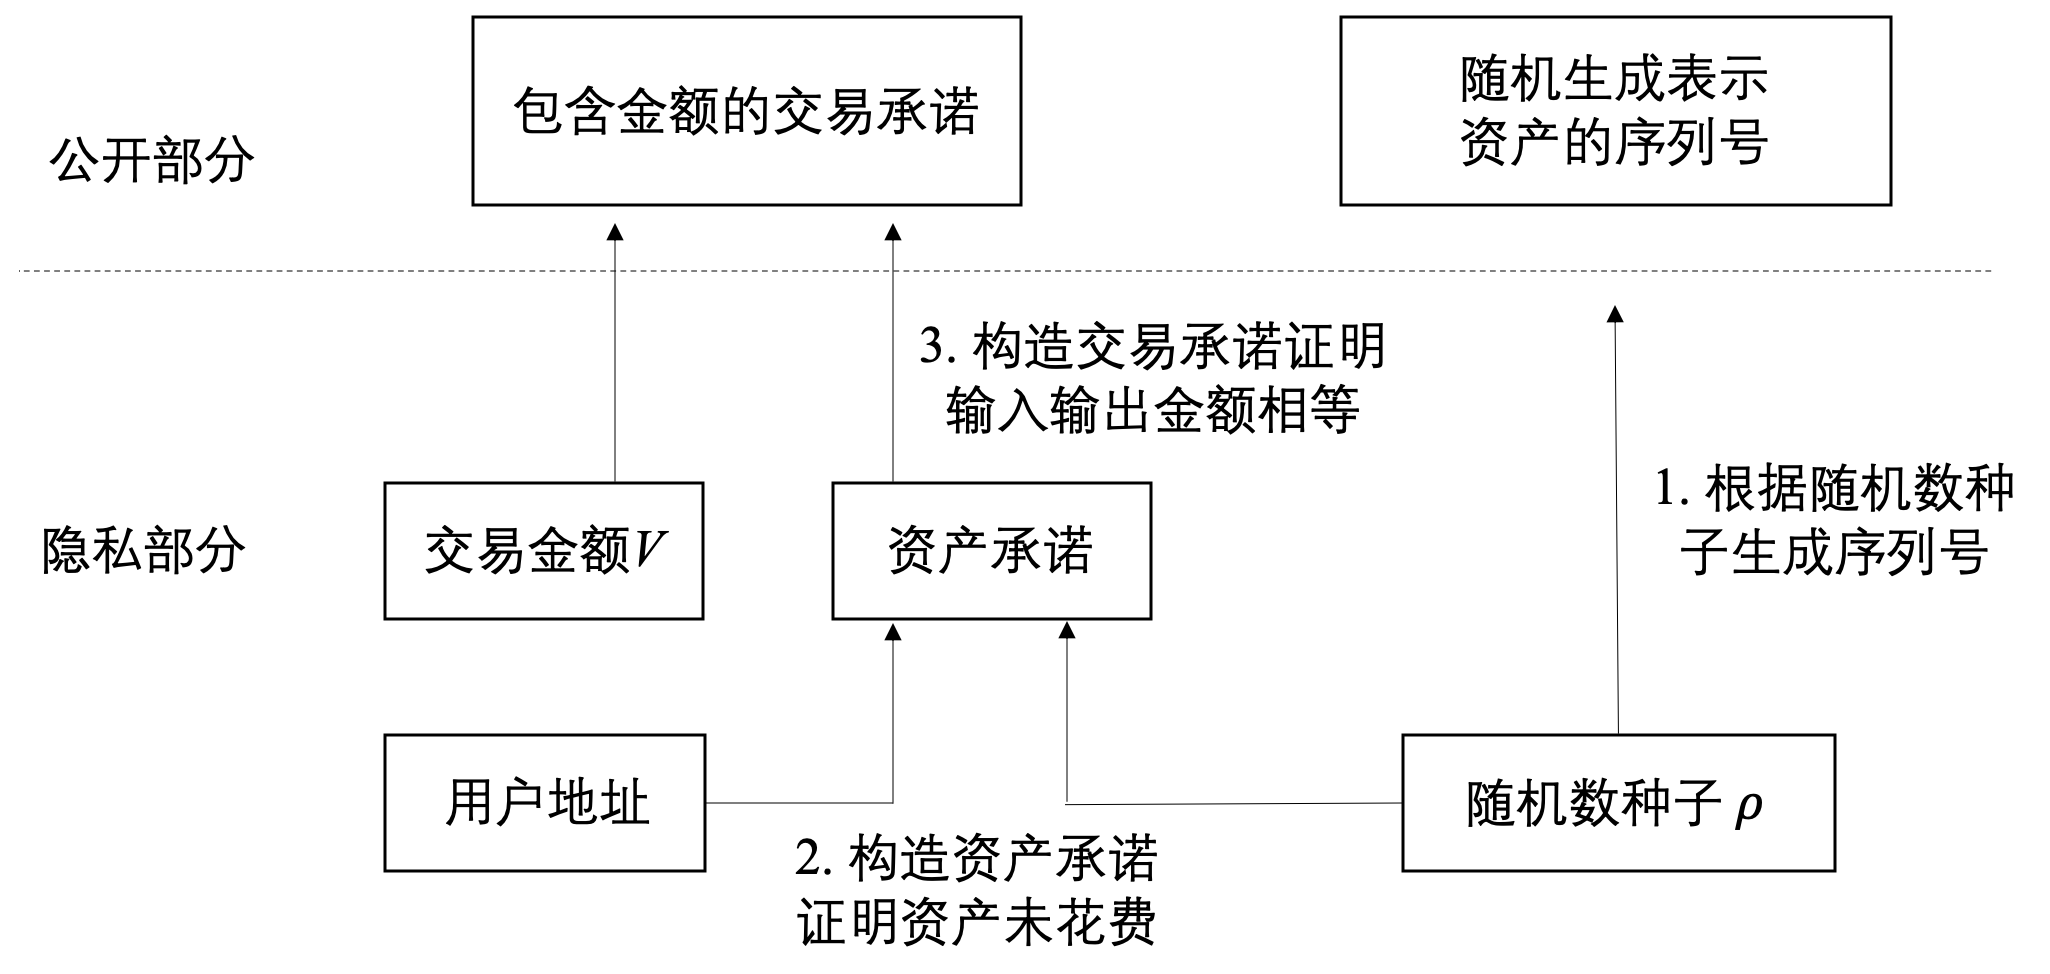
\includegraphics[width=10cm]{figures/zerocash.png}
\caption{ZeroCash协议中铸币交易的构造过程}
\label{fig:zerocash}
\end{figure}

2014年,Eli等人基于Pinocchio系统提出ZeroCash项目[23],该项目利用Pinocchio系统实现的zk-SNARKs技术构造交易。用户可以隐藏交易的发起者、接受者、交易金额等隐私信息,验证节点仍可以直接验证交易正确性。该协议与ZeroCoin同样包含铸币交易与花费交易,通过销毁资产生成私密资产,花费私密资产时其他用户无法判断该资产的来源。ZeroCoin协议中私密资产每次花费都会变为公开资产,而ZeroCash协议的私密交易可以使得输出资产也保持私密。

ZeroCash 协议可以隐藏更多的交易信息包括交易金额和接收方地址,这对于用户隐私提供了更强的保护,同时也便于用户在使用中自由设定交易金额不必收到ZeroCoin中固定币值的约束。但是,ZeroCash的缺点同样在于需要可信第三方在系统初始化阶段生成初始化的公共参数和私密参数,其中私密参数必须删除否则会直接影响到整个系统的安全,因此又被称为“有毒废料”。为了解决zk-SNARK技术中存在的依赖可信方进行启动阶段的问题,2018年, Eli等人[28]进一步提出了可扩展的透明零知识证明(zk-STARK, zero-knowledge Scalable Transparent ARguments of Knowledger)技术,并在此基础上实现了Aurora方案[29]。该技术同样先将任意计算的验证转化为多项式相等的验证,然后利用插值证明该多项式计算结果极大概率符合要求。但为了防止恶意攻击者伪造更高阶的多项式通过测试,zk-SNARK技术需要依靠可信创始方生成的密码参数,zk-STARK采用FRI(Fast Reed — solomon Interactive oracle proof of proximity)协议证明多项式的阶小于特定值。zk-STARK技术一方面达到了启动阶段的透明性,不需要依赖可信的创始方,另一方面也减少了验证证明需要的时间,提升了协议扩展性。不足之处在于生成的证明需要消耗更大的存储空间。

\subsubsection{环签名技术}

在某些场景下,一个团队中的成员希望以团队名字对消息进行数字签名,并且保护自己的身份隐私不泄露。1991年,Chaum等人[53]首次提出群签名的概念,该技术允许团队中的成员以团队名义对消息进行数字签名,其他人只能验证签名者是否属于该团队中,从而保护个人隐私。但群管理员可以披露签名者的具体身份。在此基础上,2001年,Rivest等人[54]提出了环签名的概念,环签名技术是一种简化的群签名技术,与群签名技术不同的是,该技术方案中不需要群管理员进行管理,不需要群创建过程,也没有人能对签名者身份进行披露,用户可以自由选择成员集合,并且利用自己的私钥和集合中其他成员的公钥对消息进行签名。

环签名技术主要有以下特征:

\begin{enumerate}
	\item 群中任何成员可以独自发布正确签名。
	\item 群中任何成员只知道自己是否发起该签名,群外成员只能知道该签名者是否属于群内。
\end{enumerate}

2013年,Saberhagen等人基于环签名技术提出了CryptoNote协议[24],该协议提出了匿名电子现金系统在隐私方面需要满足的两大特性,并针对这两大特性设计协议。

\begin{enumerate}
	\item 不可追踪性:对每个交易输入,所有可能的交易发起者都是等可能的。
	\item 不可链接性:对任意两个交易输出,不能证明他们是否发送给同一用户。
\end{enumerate}

其中不可追踪性保护交易发起者的隐私,不可链接性保护交易接受者的隐私,这两大特性可以保障用户的交易隐私安全。为了实现不可追踪性,CryptoNote协议采用环签名技术对交易输入进行签名,交易发起者选择多个相同输出金额的资产,构造合法的环签名,隐藏真实的交易发起者。同时,为了防止双花攻击,该协议在可追踪环签名[55]的基础上实现了“一次性环签名”,避免同一资产被花费多次。另一方面,该协议采用一次性公私钥对实现不可链接性。
	
为了满足不可链接性,发送给同一接受者的不同资产需要发送到不同的地址,在传统区块链系统中,这需要接受者每次都生成新地址并从私密通道传递给发送者。在实际应用中,这给交易双方都带来不便。为了解决这一问题,CryptoNote采用了一次性公私钥对的方式,发起者可以根据接受者的长期公钥生成新的一次性公钥,新公钥只有接受者能计算出对应的私钥,并且不能被其他用户关联到接受者的长期公钥。这样在保证了同一接受者每次交易存在不同接受地址的同时,发送者不需要接受者告知新公钥,可以独立构造交易。


\begin{figure}[ht]
  \centering%
  \subcaptionbox{发起者生成一次性公钥,发起交易\label{fig:one-time-gen}}
    {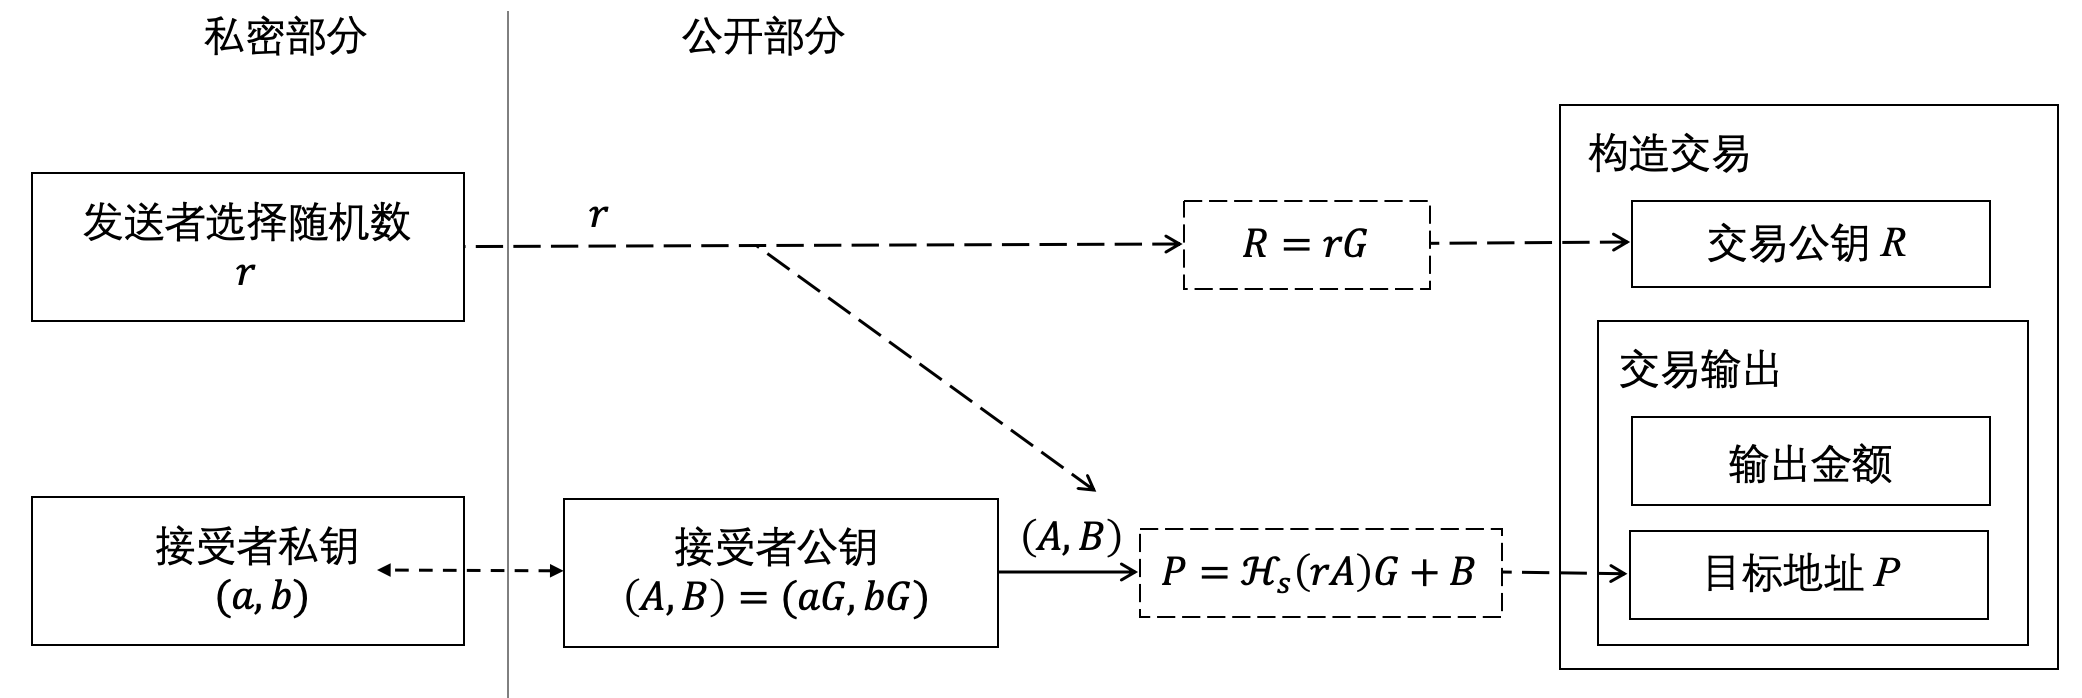
\includegraphics[width=7cm]{figures/one-time-gen.png}}%
  \hspace{4em}%
  \subcaptionbox{接受者生成一次性私钥,检查交易\label{fig:one-time-verify}}
  	{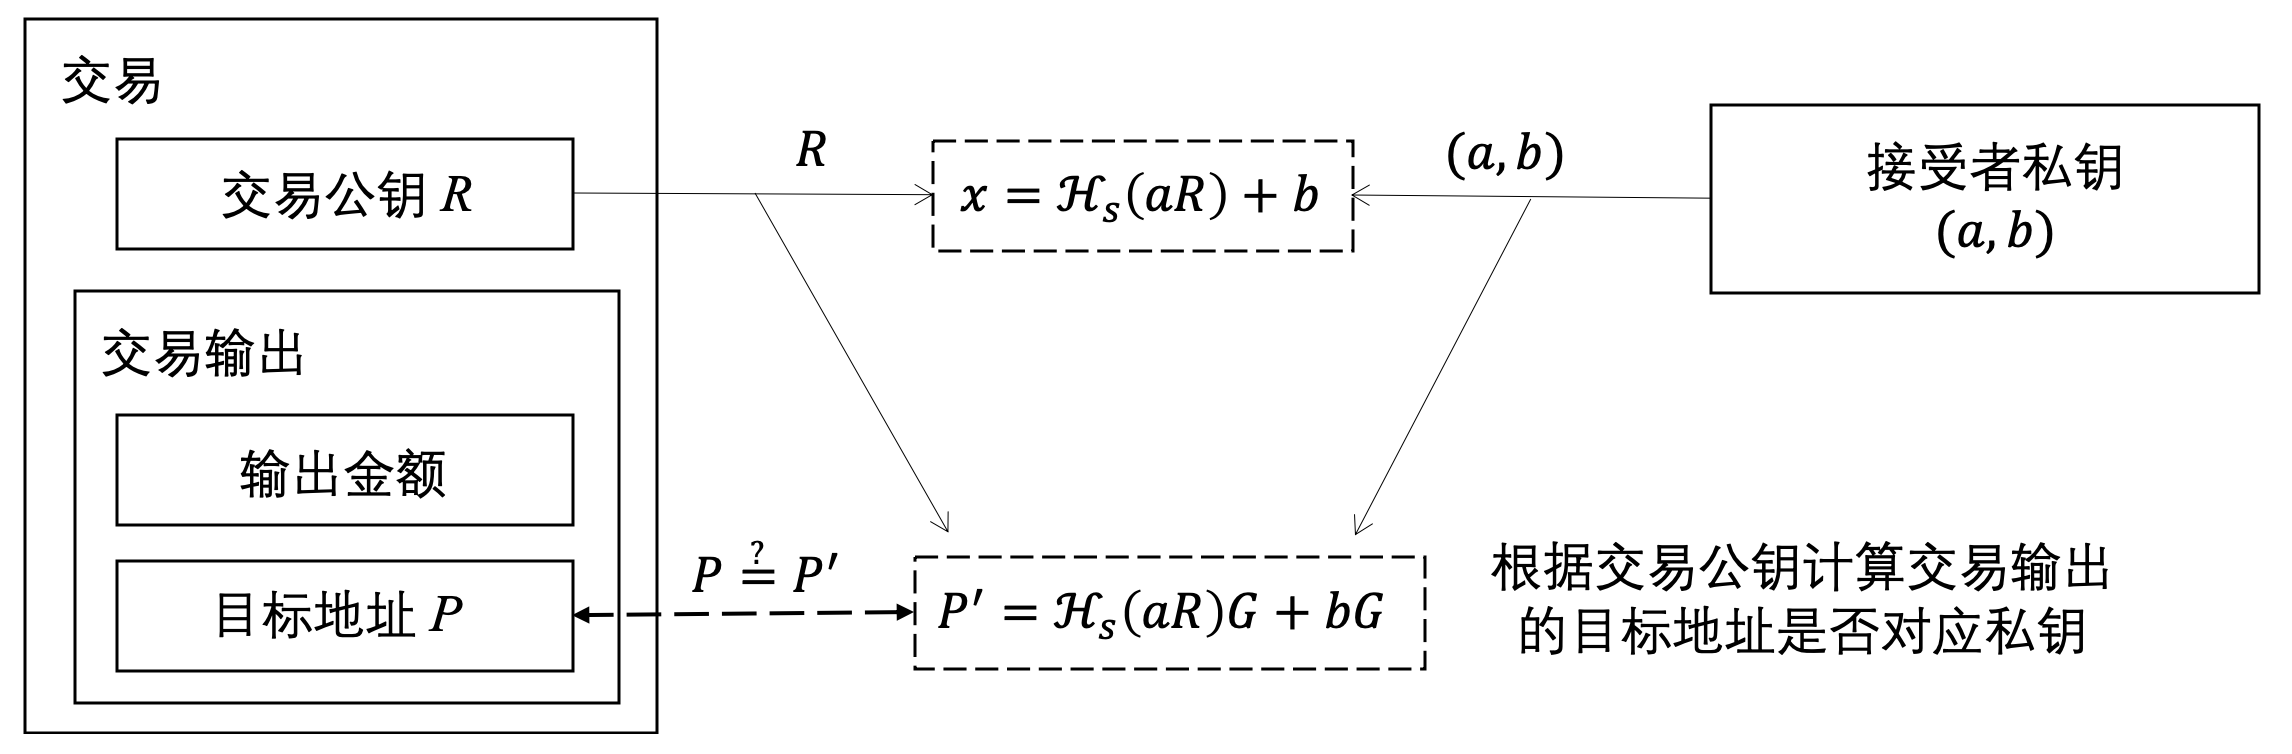
\includegraphics[width=7cm]{figures/one-time-verify.png}}
\caption{使用一次性公私钥对交易流程}
\label{fig:one-time-key}
\end{figure}

采用一次性公私钥对完成交易的流程如图\ref{fig:one-time-key},分为交易发起者生成交易与接受者检查交易两部分。交易发起者生成随机数与接受者公钥计算一次性公钥,作为交易的目标地址,并在交易中公布随机数对应的交易公钥。接受者用私钥与交易公钥计算一次性公钥判断是否为交易目标地址,如果匹配则能用私钥对该输出资产进行签名并花费。

为了满足不可追踪性,在发起交易的时候,CryptoNote协议改进可追踪环签名技术,在一次性公私钥对的基础上采用一次性环签名技术保护交易发送者隐私。一次性环签名同样分为生成签名与验证签名两阶段,并利用私钥哈希值作为快照保证资产对应私钥只进行过一次花费。

CryptoNote协议在交易中采用一次性公私钥对保护了接收方的隐私,采用一次性环签名保护了发送方的隐私。但CryptoNote协议采用环签名保护用户隐私的主要问题在于用户隐私依赖于选择的公钥集合,一旦集合中的其他用户公开使用了资产或发生隐私泄漏,导致输出被关联到对应地址,则该用户的地址关联情况也会被攻击者分析得出,导致隐私泄漏[56]。此后ByteCoin[57],Boolberry[58],DigitalNote[59]等一系列区块链项目都采用了CryptoNote作为底层框架来保护用户隐私。其中应用较为广泛的是Surae等人提出的Monero项目[60],该项目通过强制每笔环签名交易至少包含2个额外资产的方式,解决上述隐私泄漏的风险,增强了用户的长期匿名性[61]。

\subsubsection{机密交易技术}

2013年,Adam[62]提出引入同态加密技术[63]隐藏交易金额的思路,在不泄漏交易输入输出金额的具体数值的前提下,保障交易的输入输出资产金额相等。利用范围证明技术保障资产金额的数值在合法范围内,避免负数或越界的情况。2015年,Maxwell[64]对该想法进行了完善及实现,通过引入盲化因子避免了暴力枚举攻击,提出了机密交易技术(Confidential Transactions)。

机密交易技术中采用Pedersen承诺[65],在不透露交易金额的情况下使得其他节点能验证交易输入输出金额之和相等的正确性,利用椭圆曲线密码体系(ECC,Elliptic curve cryptography)[66]隐藏金额,并添加盲化因子保证在输入金额与输出金额相等的情况下,发起者才能对交易进行正确签名,同时盲化因子也能防止攻击者通过枚举暴力破解金额。为了防止负数和越界情况的出现,机密交易中采用环签名技术和盲化因子进行范围证明。但该方案采用的范围证明技术带来较大的时间复杂度和空间复杂度,为了解决这一问题,Maxwell提出一种新的环签名Borromean环签名[67]对该签名进行优化,可以提升到两倍的渐进效率。

然而,机密交易仅隐藏账本数据中的交易金额,不能隐藏交易发起者和接收者地址信息。2015年,Noether等人通过改进可链接自发匿名群签名(LSAG,Linkable Spontaneous Anonymous Group signature)技术[68],提出多层可链接自发匿名群签名(Multilayered LSAG)技术,并结合CryptoNote协议中的一次性环签名技术、一次性密钥对技术以及Maxwell提出的机密交易技术,提出了环机密交易技术[25]。该技术通过结合上述技术能同时隐藏区块链账本数据中交易金额、交易输入地址、交易输出地址。

\subsection{网络信息隐藏}

区块链系统的P2P网络中,攻击者通过部署足够多的节点监听网络中消息收发情况,可能将用户的IP地址与链上交易、地址等信息关联。因此除了对链上数据进行隔离的方法之外,为了保障区块链系统中用户IP地址的隐私,部分研究建议采用混淆网络对区块链系统进行加固,使得攻击者无法分析真正的消息发出方。现有的混淆网络主要基于两种路由技术:洋葱路由和大蒜路由,其中洋葱路由的代表项目为Tor网络,大蒜路由的代表项目为I2P网络。

\subsubsection{洋葱路由技术}

洋葱路由是一种保护网络通信的真实发送和接受节点,达成匿名通信的网络链路协议。洋葱路由通过对传输消息进行多层加密,使得路由中间节点只能知道前继节点和后继节点的IP地址,不能获取消息的真实发送节点IP与接收节点IP,保护消息发送方和接收方的真实IP不被攻击者知晓。除了出口节点外,其他中间节点也不知道消息的真实内容,保护消息内容隐私,因而只有出口节点知道自己属于出口节点,其他中间节点无法判断消息来源是客户端还是其他中转节点。

\begin{figure}
\centering
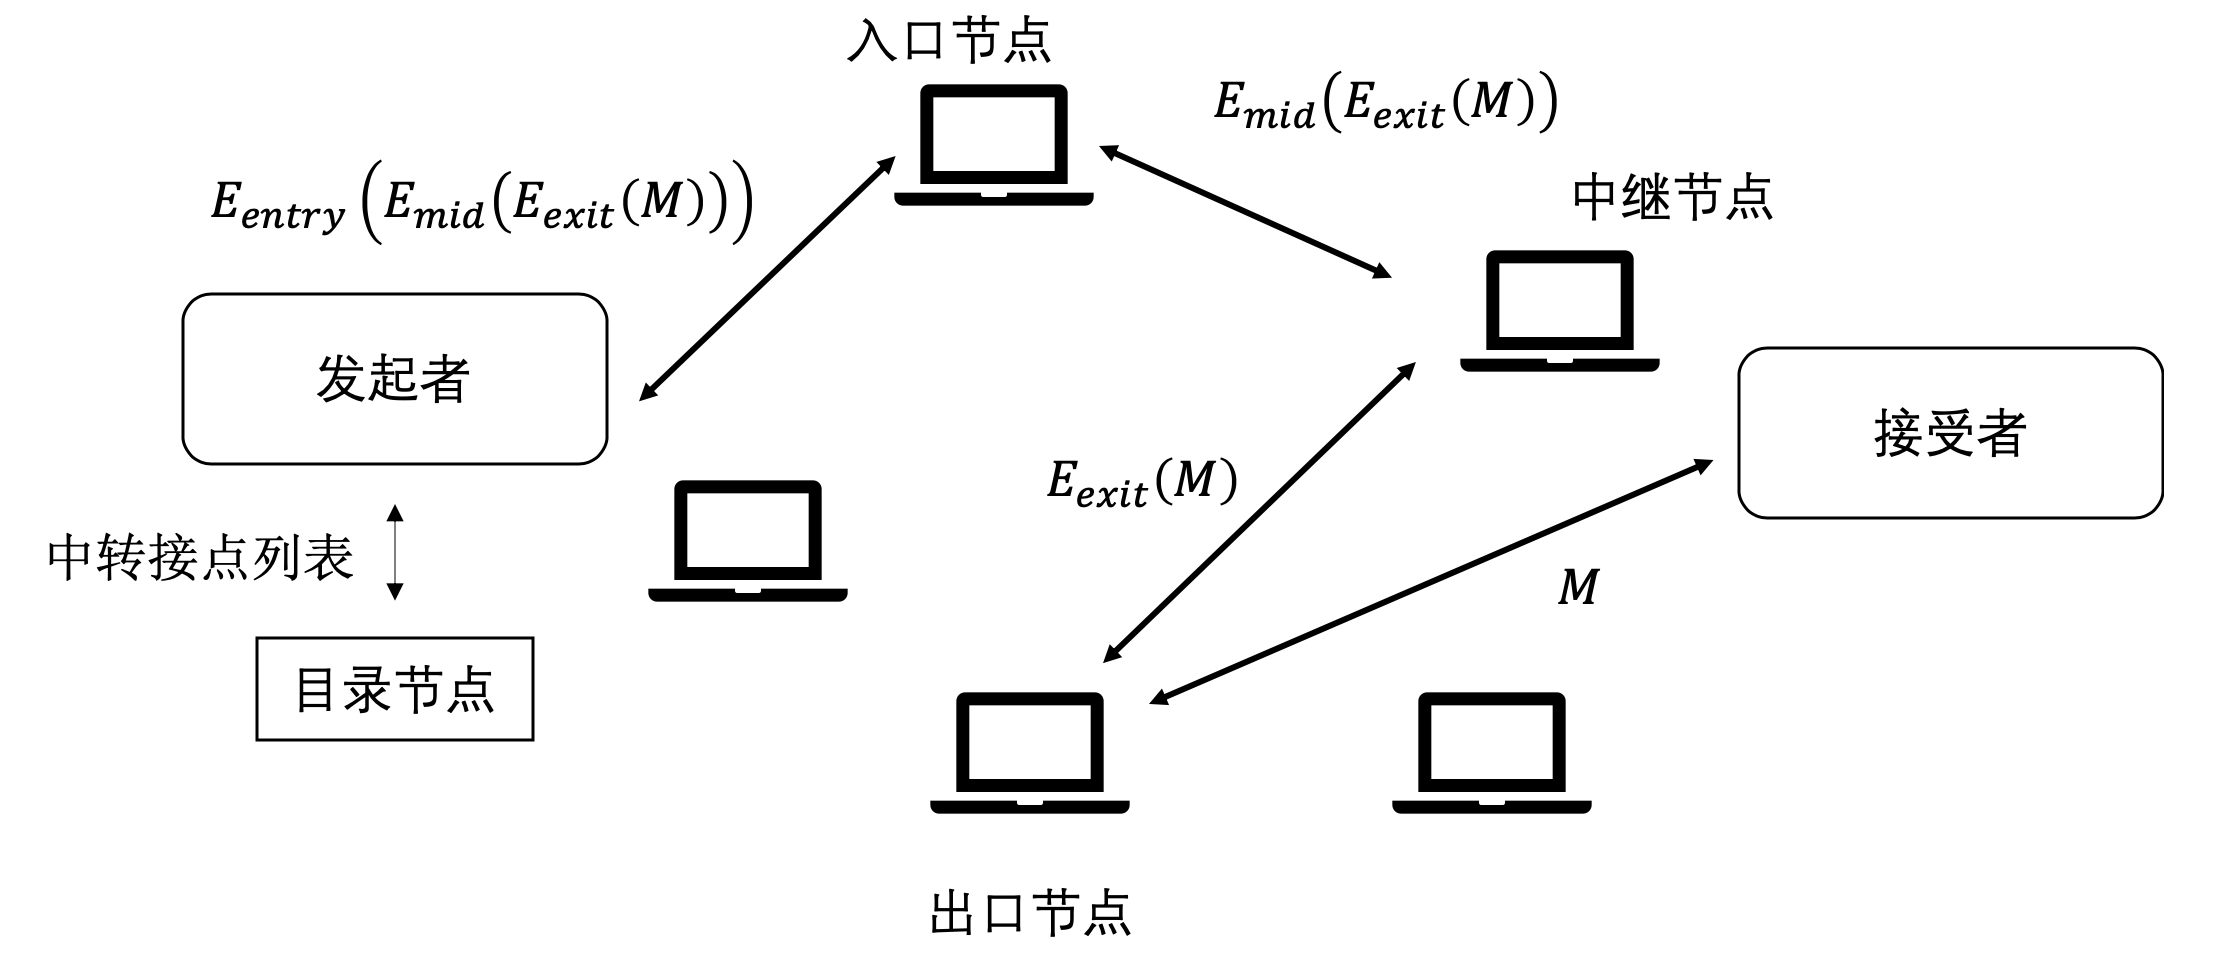
\includegraphics[width=10cm]{figures/tor.png}
\caption{Tor网络示例}
\label{fig:tor}
\end{figure}

基于洋葱路由原理的混淆网络项目主要有Tor网络[69],Tor网络建立发起者到接受者的链路主要包含以下三个阶段:

\begin{enumerate}
	\item 节点选择阶段:客户端从目录节点(directory node)提供的中转接点列表中随机选定网络中三个中转节点分别做为入口节点(Entry node)、中继节点(Middle Relay node)、出口节点(Exit Relay node)。
	\item 链路建立阶段:节点选择完成后,发起者从入口节点开始逐步建立链路。首先发起者与入口节点建立TLS链接,建立之后向入口节点发送信号,向中继节点建立链路,然后通过入口节点向中继节点发送信号,同样建立中继节点到出口节点的链路。
	\item 消息传输阶段:链路建立完成后,发起者可以通过该链路与接受者通信,所发送消息依次采用与三个中转节点协商好的会话密钥进行加密,中转节点层层解密,出口节点解密后发送给接受者。接受者返回信息沿原链路返回。
\end{enumerate}

为了增强用户隐私保护,部分比特币钱包内置了Tor网络配置,使得运行比特币钱包的节点可以通过Tor节点与比特币网络连接,从而保护节点的IP等隐私信息。采用Tor网络的比特币钱包可以在一定程度上抵抗网络监听攻击。但另一研究表明直接在Tor网络之上运行带黑名单机制的区块链项目(例如比特币)会带来安全隐患[70]。在比特币系统中,为了防止恶意节点进行拒绝服务攻击,节点设置了黑名单机制,当从某一节点接受到不合法消息后,会降低该节点信誉度,降低到0后加入黑名单,24小时内不接受该节点发送的消息。如果直接运行在Tor网络上,攻击者可以通过正常出口节点发送不合法消息给用户节点,迫使用户节点将所有正常出口节点加入黑名单,然后恶意节点通过部署自己的出口节点进行监听,这一攻击将威胁到用户身份隐私。

\subsubsection{洋葱路由技术}

尽管Tor网络采用洋葱路由技术保护通信匿名性,但是仍存在一定的安全隐患,例如流量分析攻击可以通过监听Tor网络中各节点的流量收发情况,分析网络中的流量变化情况,根据各Tor节点同一时刻的流量进出情况,判断节点间的链路关系,进而找出通信的真实发送方与接收方[71]。

为了抵抗流量分析攻击,大蒜路由将每个独立的消息称为一个蒜瓣,每个蒜瓣拥有对应的指示信息,表示该蒜瓣的类型和用途。客户端将多个蒜瓣封装成一个大蒜消息进行发送,拆分后通过不同链路传递,数据的返回采用不同的链路,同时数据往返采用的链路条数可以不同。因此基于大蒜路由的I2P网络(Invisible Internet Project)在抗流量分析攻击上比Tor网络更加安全。另一方面,I2P网络通过本地的Net DB发现节点,Net DB在每次链接其他节点时,采用Kad算法[72]进行更新,比Tor网络中的目录服务器方法有更强的安全性,但需要为此付出性能降低的代价。

\begin{figure}
\centering
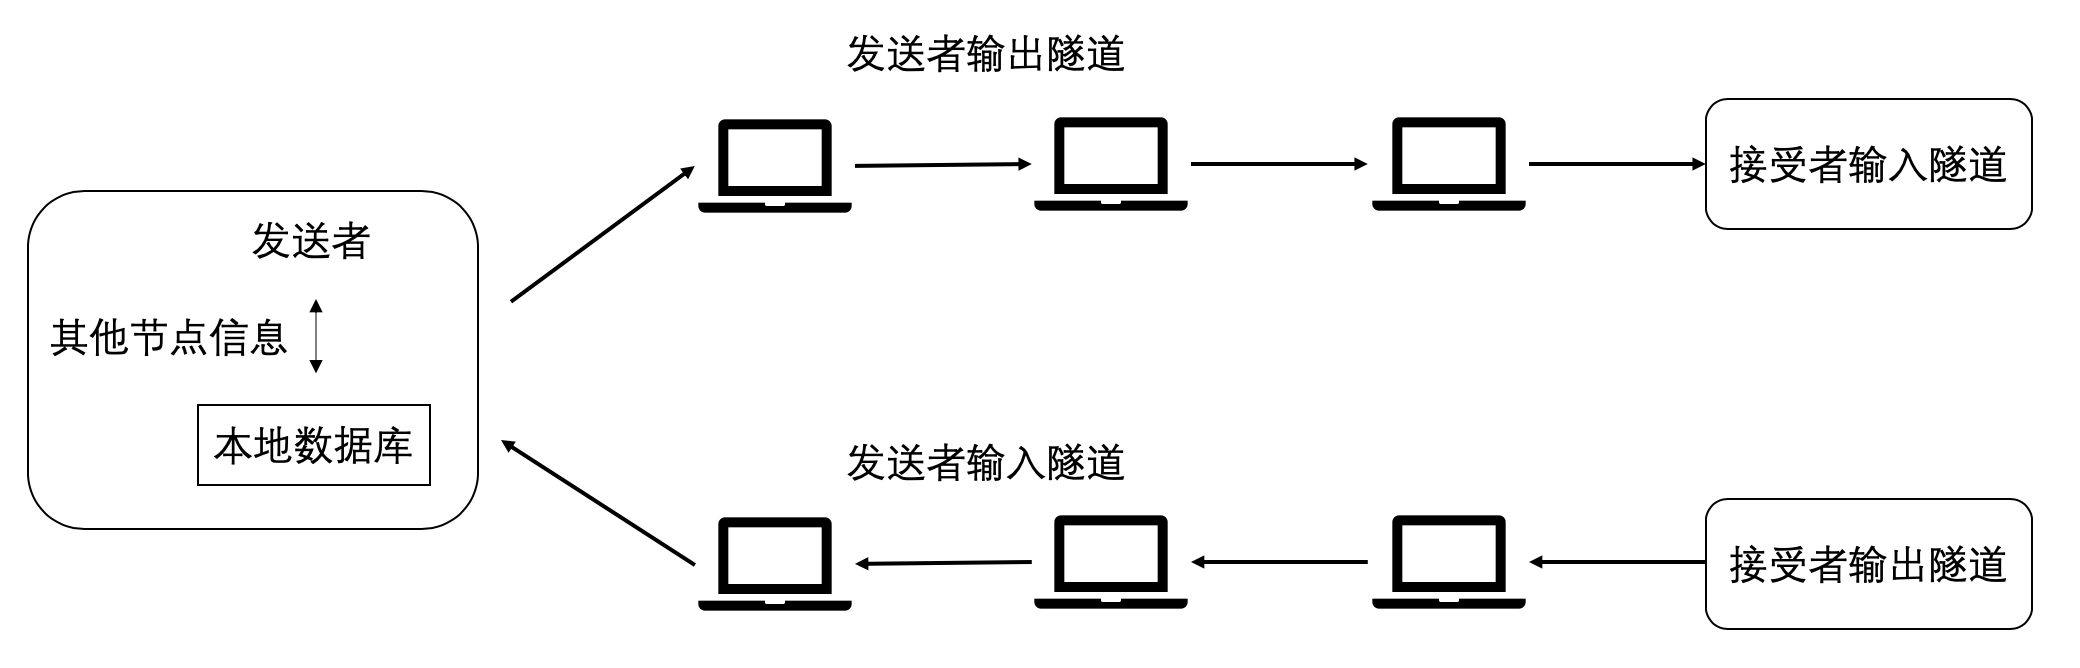
\includegraphics[width=10cm]{figures/i2p.png}
\caption{I2P网络中的隧道}
\label{fig:i2p}
\end{figure}

I2P网络中,用户通过传递可变隧道建立(VTB,Variable Tunnel Build)消息建立输入输出隧道,每个VTB消息由多个建立请求记录(BRR,Build Request Record)组成,其中每个BRR包含接受节点信息和其他相关信息。I2P网络建立隧道与Tor网络同样采用多层加密技术,但在发送消息和返回消息采用输出和输入两条不同链路,使得流量保持单向传输,通信双方的输入输出隧道将构成环路,能隐藏真实的通信节点,抵抗流量分析攻击。I2P网络通过分离链路的方式进一步隐藏了隐藏网络中流量情况,在Tor网络的基础上进一步增强了用户隐私安全。

\section{通道隔离机制}

通道隔离机制从网络层面对数据进行隔离,保护数据只对通道内节点可见。通过对账本进行隔离,每个节点只处理并存储自己所在通道的数据,防止攻击者访问数据,保护用户隐私。但是通道机制也存在一定缺陷,主要体现在区块链网络中通道部署存在一定代价,节点创建和进出通道需要进行网络配置的修改,灵活性较弱。根据被隔离数据的存放位置,通道隔离机制的实现技术可以分为链下通道隔离和多链通道隔离两大类。

链下通道隔离主要应用于高频小额交易,用户通过在区块链上记录起始的状态创建通道,随后在链下进行交易,具体数据通过合约保证安全,但不公布记录在区块链上,需要中止交易的时候再将最新的结束状态公布并记录在区块链上,终止通道并销毁历史交易记录。

多链通道隔离通过在特定节点之间构建独立通信网络作为通道,该网络中信息单独存放在子账本中,非通道内节点不能访问,同一节点可以加入多条不同通道中。多链通道隔离通过在网络层面构建子网络,实现节点通信隔离,杜绝攻击者访问隐私信息,保护用户隐私。

\subsection{链下通道隔离}

为了解决区块链账本容量有限的问题,研究者尝试将小额高频交易放在链下的微支付通道进行,仅仅将通道启动和结束的信息记录在区块链账本上。典型的微支付通道技术为比特币系统中的闪电网络技术[26]与以太坊系统中的雷电网络技术[27]。其中闪电网络技术针对基于未花费交易输出模型的密码货币,雷电网络主要针对基于账户余额状态模型的密码货币,更多利用链上合约机制。该技术主要分为两步,首先在两个节点之间构造链下双方支付通道,然后通过节点间的双方支付通道构建支付网络。

双方支付通道:在两个地址间构建可信的链下支付通道。通过将资产托管到链上合约创建支付通道,随后参与双方通过对状态更新进行签名确认进行交易,具体过程不需要记录到区块链账本中。当某一方希望中断通道时,将最新状态发布到区块链中,并赎回最新状态对应资产。
构建支付网络:在所有参与用户之间两两构建双方支付通道会带来巨大的存储资源和资产的浪费。因此在双方支付通道的基础上,用户通过已有的双方支付通道进行支付,从而构建全体用户之间的支付网络。

\subsubsection{闪电网络技术}

2016年,Poon等人提出了比特币系统中的闪电网络技术[26],该技术主要由序列到期可撤销合约(RSMC,Revocable Sequence Maturity Contract)和哈希时间锁定合约(HTLC,Hashed Timelock Contract)组成,利用RSMC实现双方支付通道,通过HTLC进一步构建支付网络。这一设计在提高比特币系统性能的同时,也通过隐藏不在链上记录用户间的小额支付保护了用户隐私。

\begin{figure}
\centering
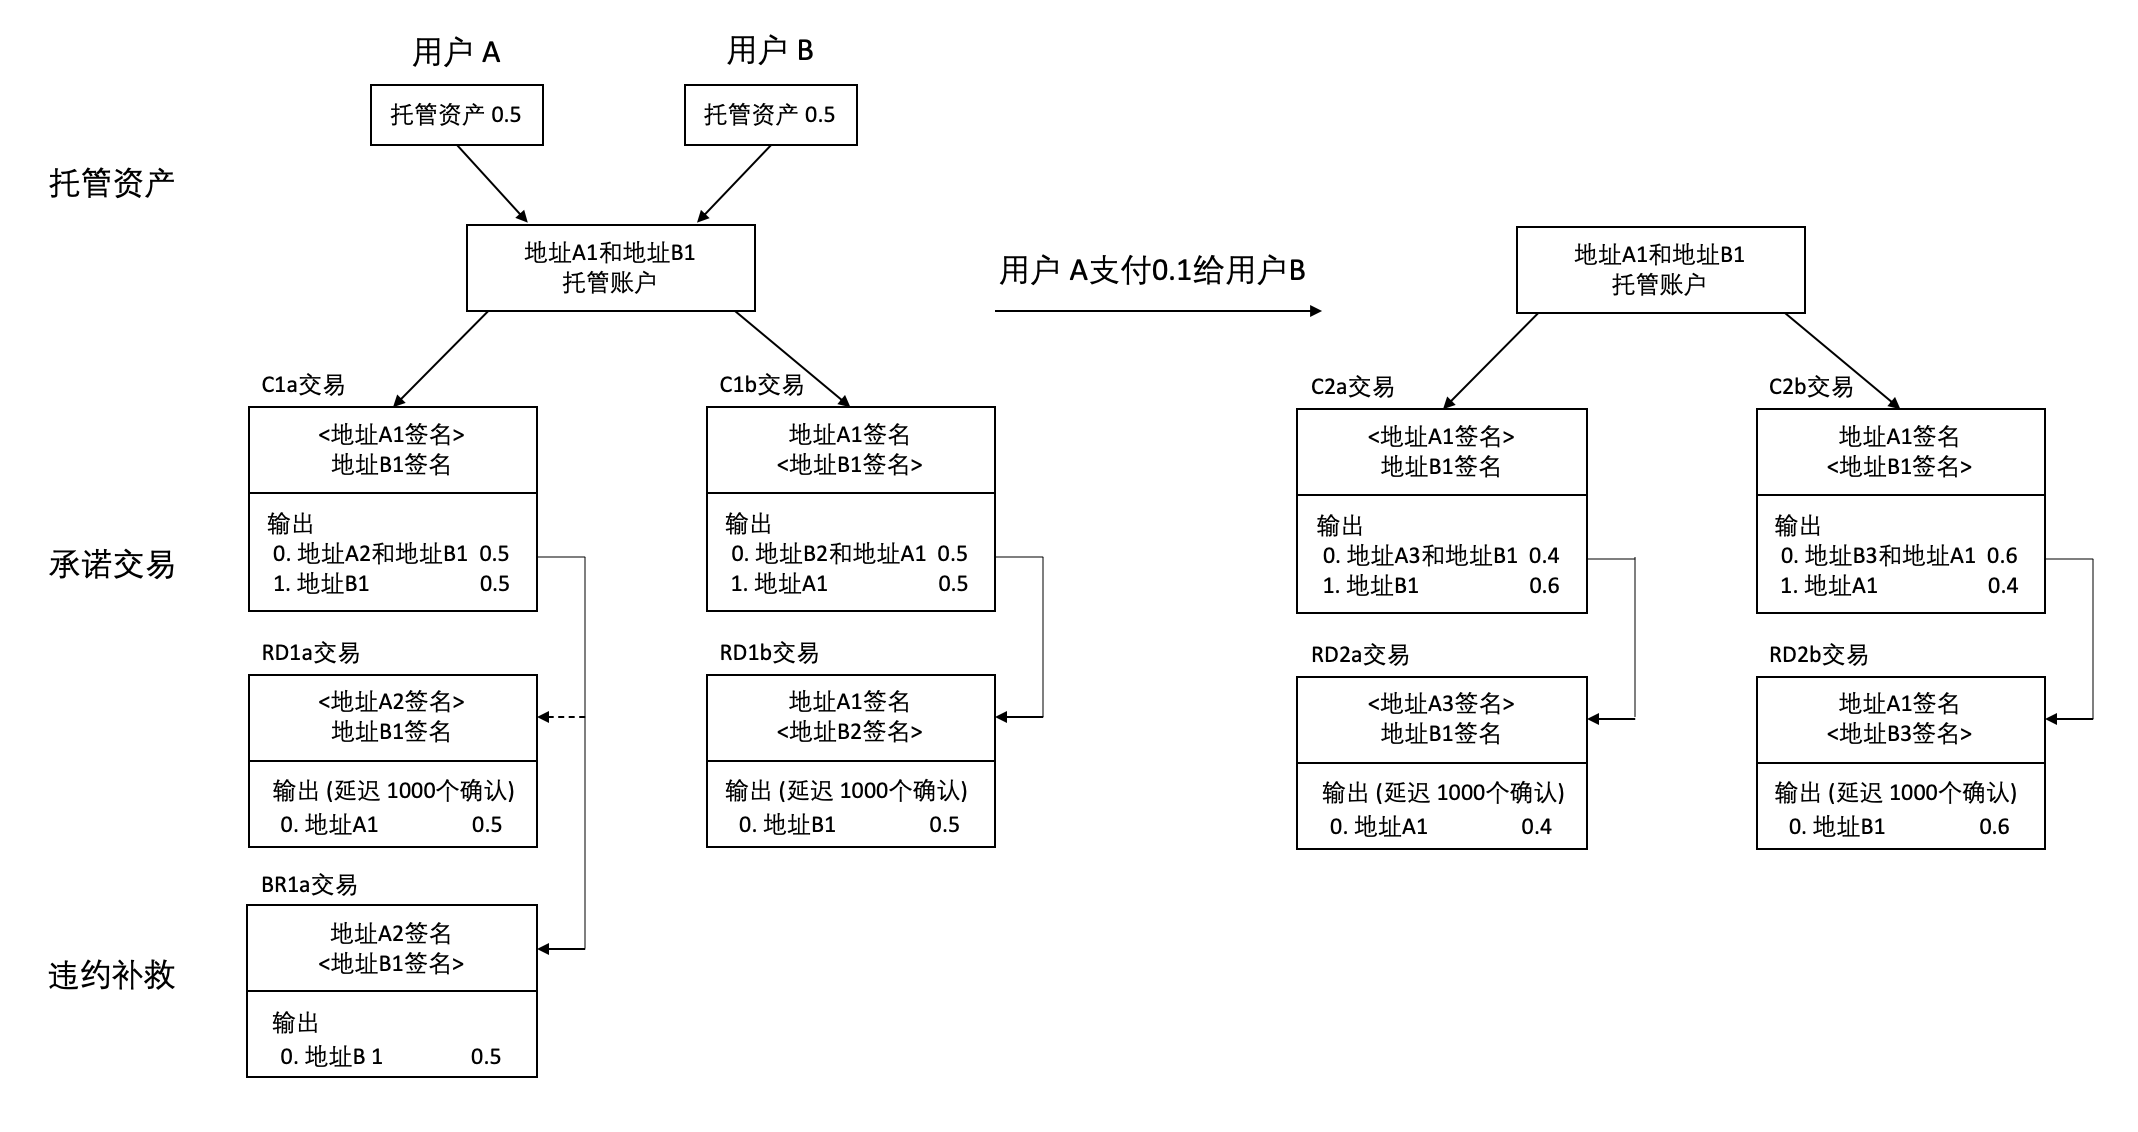
\includegraphics[width=10cm]{figures/lightning-network.png}
\caption{序列到期可撤销合约的通道创建和状态更新}
\label{fig:lightning-network}
\end{figure}

双方支付通道: 序列到期可撤销合约(RSMC)通过不断创建2/2多重签名钱包,构建双向支付通道。只在合约创建和结束时各在比特币账本上发布一次的特性,保障用户隐私。图17展示了一个具体的序列到期可撤销合约的创建及支付过程:

\begin{enumerate}
	\item 托管资产阶段:用户A和用户B双方各拿出部分资产,托管到双方签名账户,该账户的支出需要双方共同签名,此后支付阶段中支付通道的交易状态各用户花费不能超出所托管资产。但双方不对托管交易签名,更不广播到区块链网络。
	\item 构造通道阶段:用户A构造承诺交易1a(C1a,Commitment transaction 1a)和可撤销支付交易1a(RD 1a,Revocable Delivery 1a),并交给用户B签名。C1a交易用于保证在用户A单方中止通道的情况下,Bob能得到自己的托管资产。RD1a用于保证用户A能单方取回自己托管的资产,该交易带有延迟设定,若C1a被记录在第n个区块,则RD1a只能记录在第n+1000个区块之后的区块。Bob对称构造承诺交易C1b和RD1b,并交给Alice签名。双方均完成对承诺交易和可撤销支付交易的签名并交换后,各自再对托管交易进行签名并广播,合约建立完成。
	\item 支付阶段:当用户A支付0。1单位资产给用户B时,首先需要将C1a和RD1a代表的状态作废,用户A构造并签名违约补救交易(BR1a, Breach Remedy 1a),发送给用户B,因此当用户A发布C1a后,在1000个区块时间内,用户B可以发布BR1a。然后双方按照构造通道阶段中的步骤,根据支付后的余额分配情况重新构造承诺交易C2a、C2b以及可撤销支付交易RD2a、RD2b,完成状态改变。
	\item 结束阶段:当任一方用户希望结束合约时,先公布承诺交易,若另一用户未在延迟时间中公布违约补救交易,则表示该承诺交易为最终状态,该用户在延迟时间后再公布可撤销支付交易取回资产。
\end{enumerate}

\begin{figure}
\centering
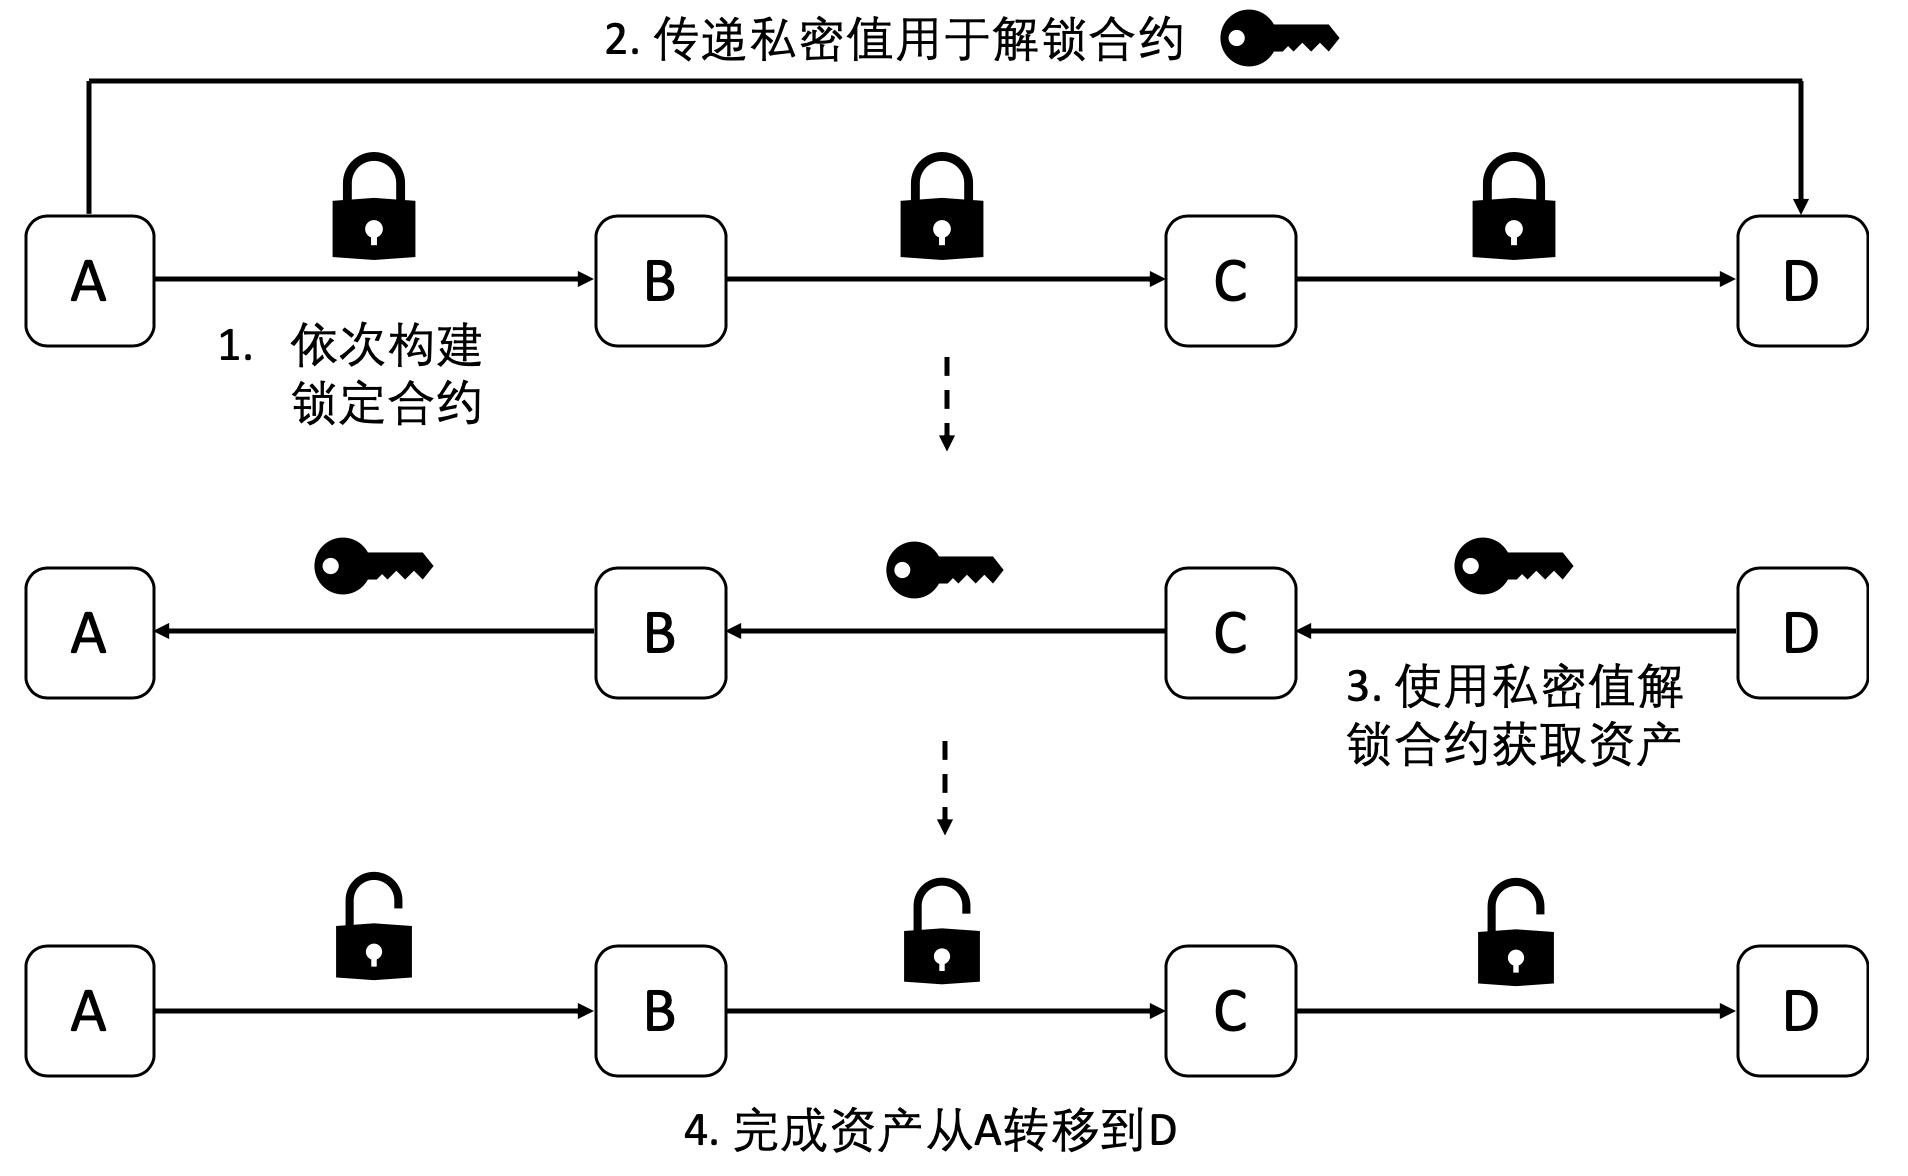
\includegraphics[width=10cm]{figures/hash-time-lock.png}
\caption{哈希时间锁合约的工作流程}
\label{fig:hash-time-lock}
\end{figure}

构建支付网络:哈希时间锁定合约(HTLC)是一类特殊的链上合约交易,通过哈希时间锁构造的链上合约保障交易双方能通过中间人进行安全交易,利用哈希原象作为支付凭证,三方参与的哈希时间锁定合约具体细节已在2。2。2节中详细介绍。多人采用哈希时间锁定合约可以帮助未建立RSMC的两个用户通过中间人建立交易通道。如图\ref{fig:hash-time-lock}所示,在AB、BC、CD之间分别存在RSMC时,AD之间可以通过已有通道完成支付。
闪电网络技术通过RSMC保障链下支付通道的资产安全性,通过HTLC减少网络中所需RSMC的数量,增强闪电网络的扩展性。利用闪电网络技术,用户之间往来的交易数据将不会记录在区块链账本上,杜绝了账本分析攻击,极大保障了用户的账本隐私安全。

\subsubsection{雷电网络技术}

在闪电网络技术的基础上,雷电网络技术[27]基于以太坊系统的智能合约机制提供更加便捷的链下支付通道。雷电网络同样分为构建双方支付通道和多方支付网络两部分,利用图灵完备的智能合约语言,简化了闪电网络中序列到期可撤销合约(RSMC)和哈希时间锁定合约(HTLC)的实现方式。

双方支付通道:雷电网络中的支付通道主要分为合约构建、余额证明、链下支付、合约撤销几个阶段。合约构建阶段由参与者为特定通道创建智能合约并发布到区块链账本。余额证明阶段中,通道中的交易双方通过向合约账户进行转账作为资产抵押,此后通道中的交易额度不可以超过证明的资产数量,保证交易双方有偿还债务的能力。完成证明后,链下支付阶段中,交易双方根据合约规定的格式,通过对更新的交易状态签署新的余额证明完成链下支付,每一次状态消息都附加上递增的序列号。闪电网络中每次记录的是新的余额状态,而雷电网络中记录的是更新的资产变化。当某一方希望中断支付通道时,停止签名新的状态消息,将当前的状态消息发送给智能合约。在一定时间内,如果合约未收到序列号更大的状态消息,则进行合约撤销,根据最新接受的状态消息返回资产到各参与者账户。

\begin{figure}
\centering
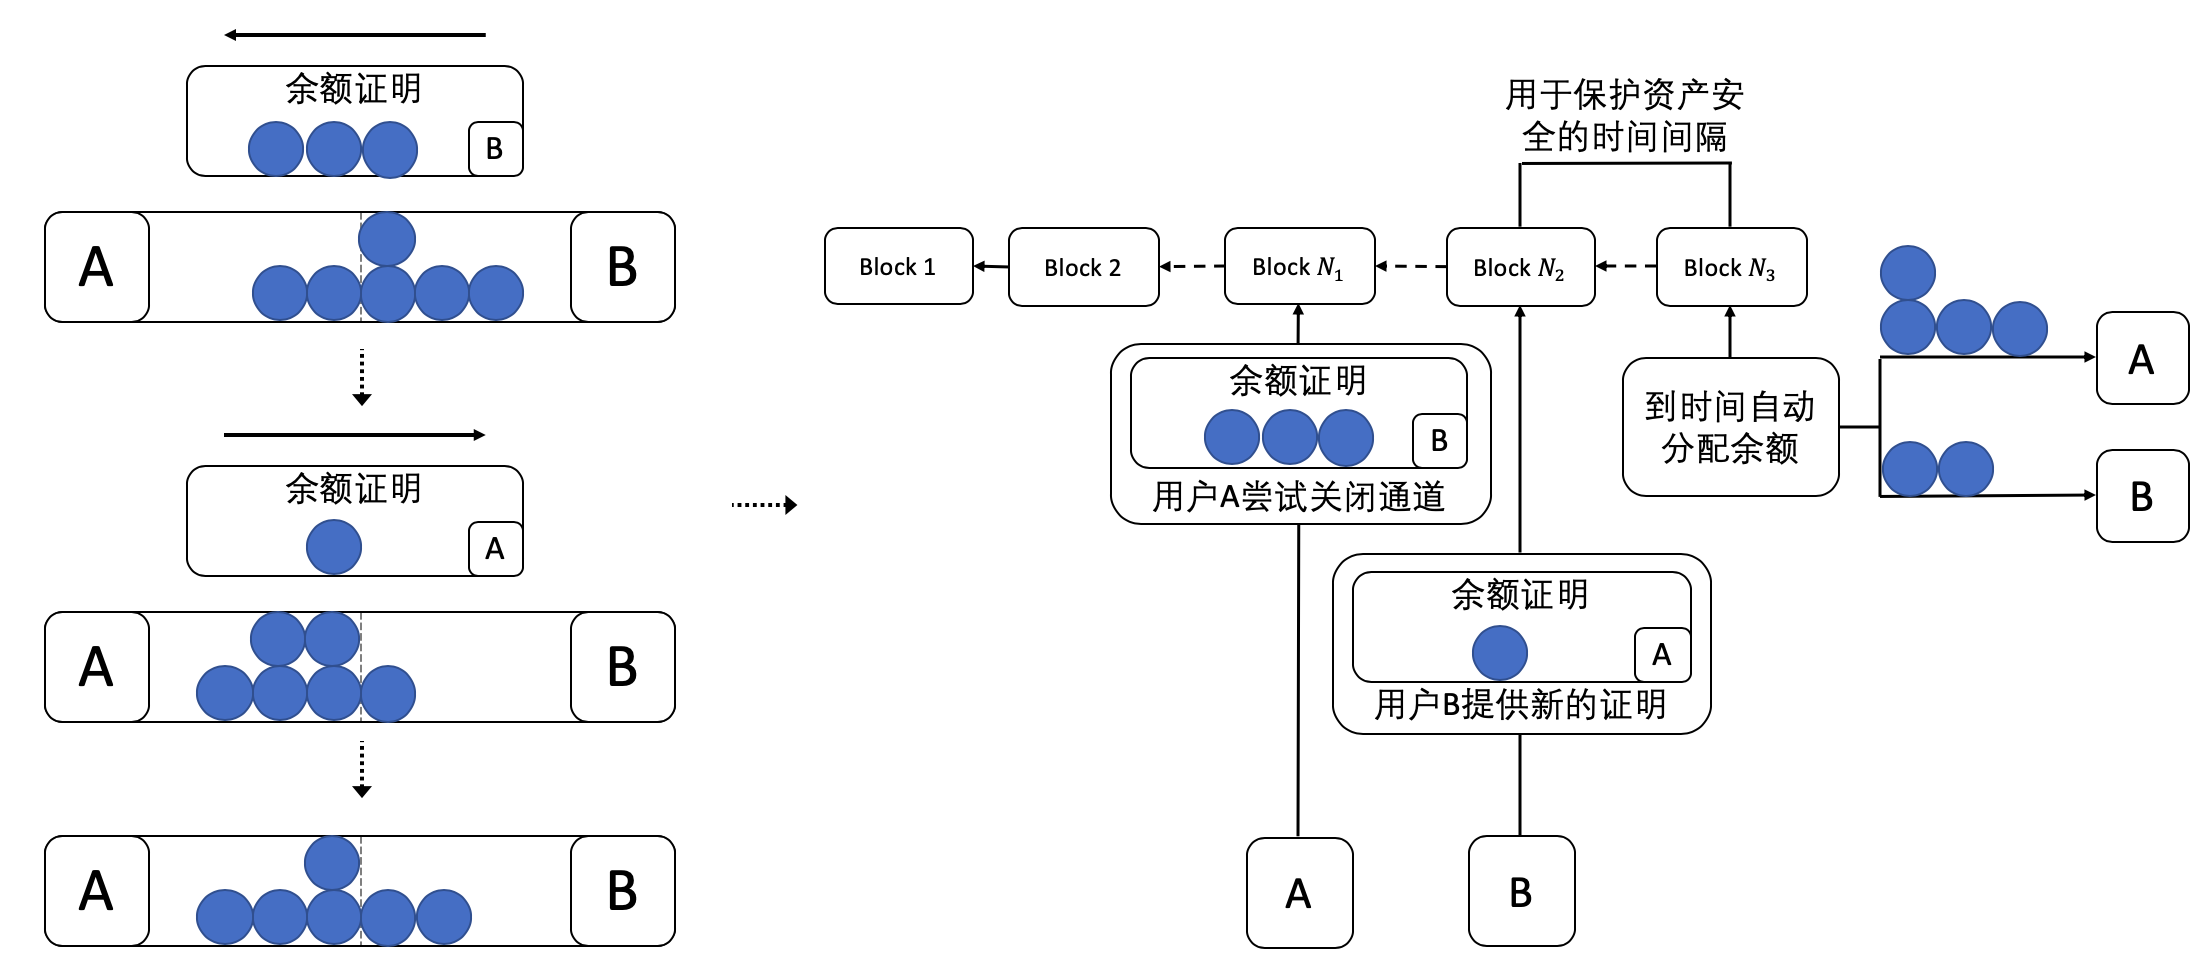
\includegraphics[width=10cm]{figures/raiden-channel.png}
\caption{雷电网络技术的支付通道示例}
\label{fig:raiden-channel}
\end{figure}

如图\ref{fig:raiden-channel}所示,第一步用户B向用户A先支付3个币,第二步用户A向用户B支付1个币。之后用户A尝试使用第一步的余额证明关闭通道,在限定时间内用户B提供新的余额证明,保证最终余额分配是按照最新状态进行。

多方支付通道:由于闪电网络技术中的HTLC存在中间用户与收款用户合谋损害付款用户资产安全性的风险,例如当用户A通过中间用户C向用户B进行支付,用户A发布向用户C支付的锁定合约后,用户C假装离线,用户A重新选择中间用户D完成支付。此时若仍在AC之间合约有效期内,用户B可以提供私密值使得用户C获取合约AC锁定的资产。为了解决这一问题,雷电网络技术在收据哈希锁(receipt hash lock)和时间锁(time hash lock)之外增加重试哈希锁(retry hash lock),该锁用于中间用户离线导致付款人需要改变支付路径的情况。雷电网络技术中的三方支付通道过程中同样由收款用户创建哈希锁并保留哈希原像作为解锁私密值。付款用户构造重试哈希锁同样保留哈希原像,并使用收到的收据哈希锁和重试哈希锁构造支付交易。等待中间用户正确发布支付后再将重试哈希锁的私密值发送给收款用户用于获取资产。若中间用户离线需要更换支付路径,则将旧交易作废,重新构造重试哈希锁,保障付款用户资产安全。

\subsection{多链通道隔离}

多链通道隔离技术在同一区块链系统中维护多个区块链账本,其中不同节点群体维护特定子区块链,通过设置访问控制机制保障子区块链数据隐私安全。

目前较为成熟的多链通道技术主要为HyperLedger Fabric项目[4]中的通道技术,通道技术主要通过在不同团队的内部节点间分别独立构建区块链,保护内部数据的隐私安全。分片技术将同一区块链账本拆分为多个分片进行维护,各分片只负责维护不同的账户信息以及事务数据,不需要验证全局的账本信息。在必要情况下分片之间需要进行通信。多通道技术在不同节点间构建互相隔离的通道,维护各自的独立账本,不同通道之间不需要进行通信,因此更强地保护用户隐私数据。

在实际的应用场景中,不同节点具有不同的链下身份,需要完成不同的业务需求,因而会根据业务组成不同的团队进行合作。为了保护同一团队内部节点间的隐私数据,多通道技术通过在不同团队的内部节点间分别独立构建区块链,维护账本数据,保护内部数据的隐私安全。多通道技术主要包含以下机制:

\begin{itemize}
	\item 身份管理:管理各节点身份授权及认证机制,持有不同身份的节点拥有相应权限。
	\item 通道管理:管理通道建立、维护、销毁的整个生命周期。
	\item 事务管理:管理通道内事务的发布、排序、记录等操作。
\end{itemize}

\begin{figure}
\centering
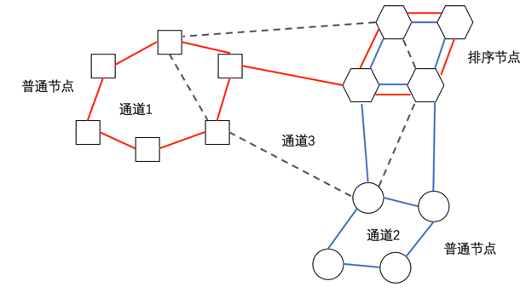
\includegraphics[width=10cm]{figures/hyper-channel.png}
\caption{超级账本通道机制}
\label{fig:hyper-channel}
\end{figure}

2017年,HyperLedger Fabric项目更新1.0版本并增加了通道机制。网络中的若干节点可以通过网络配置搭建通道,在同一通道中的节点共同维护子账本数据,通道中传输的数据不被通道外的用户接收。而某一节点可以根据自己的实际需求加入多个通道,实现了商业场景下的不同业务数据隔离。

综上所述,通道隔离技术在网络层面进行消息隔离,通过限制消息的传播范围保护用户隐私。在非许可链系统中,区块链账本对所有节点公开,因此通道主要以链下通道的形式存在,用户通过构建链下通道保护账本数据隐私,同时利用公有链账本记录通道的开启和结束保护交易安全。而在许可链系统中,主要采用传统的授权与认证技术,由于存在访问权限的设计与管理,网络配置有了更多的选择,通常采用多链机制,根据应用需要构建不同的子区块链。

\section{小结}

随着区块链技术的成熟与众多区块链系统的广泛使用,以及未来区块链技术将在更多的领域中发挥作用,区块链系统中的用户隐私威胁将会成为更加重要的研究问题。本章将现有的隐私保护技术归纳总结为地址混淆、信息隐藏、通道隔离三类机制,并详细介绍了各类隐私保护机制的原理、特征以及不同的实现方式。现有的各类隐私保护机制及实现技术从不同方面保护区块链隐私,但存在安全性、性能、扩展性等方面的不足。
